% Options for packages loaded elsewhere
\PassOptionsToPackage{unicode}{hyperref}
\PassOptionsToPackage{hyphens}{url}
%
\documentclass[
]{book}
\usepackage{amsmath,amssymb}
\usepackage{iftex}
\ifPDFTeX
  \usepackage[T1]{fontenc}
  \usepackage[utf8]{inputenc}
  \usepackage{textcomp} % provide euro and other symbols
\else % if luatex or xetex
  \usepackage{unicode-math} % this also loads fontspec
  \defaultfontfeatures{Scale=MatchLowercase}
  \defaultfontfeatures[\rmfamily]{Ligatures=TeX,Scale=1}
\fi
\usepackage{lmodern}
\ifPDFTeX\else
  % xetex/luatex font selection
\fi
% Use upquote if available, for straight quotes in verbatim environments
\IfFileExists{upquote.sty}{\usepackage{upquote}}{}
\IfFileExists{microtype.sty}{% use microtype if available
  \usepackage[]{microtype}
  \UseMicrotypeSet[protrusion]{basicmath} % disable protrusion for tt fonts
}{}
\makeatletter
\@ifundefined{KOMAClassName}{% if non-KOMA class
  \IfFileExists{parskip.sty}{%
    \usepackage{parskip}
  }{% else
    \setlength{\parindent}{0pt}
    \setlength{\parskip}{6pt plus 2pt minus 1pt}}
}{% if KOMA class
  \KOMAoptions{parskip=half}}
\makeatother
\usepackage{xcolor}
\usepackage{longtable,booktabs,array}
\usepackage{calc} % for calculating minipage widths
% Correct order of tables after \paragraph or \subparagraph
\usepackage{etoolbox}
\makeatletter
\patchcmd\longtable{\par}{\if@noskipsec\mbox{}\fi\par}{}{}
\makeatother
% Allow footnotes in longtable head/foot
\IfFileExists{footnotehyper.sty}{\usepackage{footnotehyper}}{\usepackage{footnote}}
\makesavenoteenv{longtable}
\usepackage{graphicx}
\makeatletter
\def\maxwidth{\ifdim\Gin@nat@width>\linewidth\linewidth\else\Gin@nat@width\fi}
\def\maxheight{\ifdim\Gin@nat@height>\textheight\textheight\else\Gin@nat@height\fi}
\makeatother
% Scale images if necessary, so that they will not overflow the page
% margins by default, and it is still possible to overwrite the defaults
% using explicit options in \includegraphics[width, height, ...]{}
\setkeys{Gin}{width=\maxwidth,height=\maxheight,keepaspectratio}
% Set default figure placement to htbp
\makeatletter
\def\fps@figure{htbp}
\makeatother
\setlength{\emergencystretch}{3em} % prevent overfull lines
\providecommand{\tightlist}{%
  \setlength{\itemsep}{0pt}\setlength{\parskip}{0pt}}
\setcounter{secnumdepth}{5}
\usepackage{booktabs}
\ifLuaTeX
  \usepackage{selnolig}  % disable illegal ligatures
\fi
\usepackage[]{natbib}
\bibliographystyle{apalike}
\usepackage{bookmark}
\IfFileExists{xurl.sty}{\usepackage{xurl}}{} % add URL line breaks if available
\urlstyle{same}
\hypersetup{
  pdftitle={The Vile Deeds of Christman Grippertenius},
  pdfauthor={Theophrastus Bombastus},
  hidelinks,
  pdfcreator={LaTeX via pandoc}}

\title{The Vile Deeds of Christman Grippertenius}
\author{Theophrastus Bombastus}
\date{2025-01-09}

\begin{document}
\maketitle

{
\setcounter{tocdepth}{1}
\tableofcontents
}
\chapter*{Title Page}\label{title-page}
\addcontentsline{toc}{chapter}{Title Page}

\begin{center}\includegraphics[width=1.2\linewidth]{graphics/wiki_Christeman} \end{center}

\begin{quote}
``Die erst von dem Erschrocklichen Mörder Peter Nirschen/ wie er gericht und was er bekennt hat/ In dem 1581. Jahr zu Nüwen Marckt den 16. Septembris. Im Thon/ Es geht ein frischer Sommer daher. Die ander von einem Mörder Christman Gniperdoliga genannt/ welcher von seiner jugendt auff 964. Mörd gethan hat/ Im Thon Hilff GOtt das mir gelinge \ldots{}''

\emph{Dreyerley Neüwezeitung. in Gesangweiß} \href{https://collections.thulb.uni-jena.de/receive/HisBest_cbu_00033564}{Link}
\end{quote}

This adventure is loosely inspired by the crimes of \textbf{Christman Grippertenius} and his associates \textbf{Peter Stumpp} and \textbf{Peter Niers}.

The adventure is meant for a party of 4-6 \textbf{Level 4-8} characters. The adventure is written for \textbf{Advanced OSE} and was playtested with those rules. It should be equally usable with AD\&D/OSRIC, Swords \& Wizardry, LotFP or similar systems.

The player characters will confront a group of murderers that has been terrorizing the region of Bergkessel. The main inspiration for the adventure are the historical stories and murder ballads about Christman Genipperteinga,\footnote{see \href{https://en.wikipedia.org/wiki/Christman_Genipperteinga}{Wikipedia} for a quick overview.} Peter Niers,\footnote{see \href{https://en.wikipedia.org/wiki/Peter_Niers}{Wikipedia} for a quick overview.} and Peter Stumpp.\footnote{see \href{https://en.wikipedia.org/wiki/Peter_Stumpp}{Wikipedia} for a quick overview.} The adventure does not strive for historical accuracy, merely to provide an engaging dark fantasy scenario for OSR gaming. If you'd like to read more about each of these three individuals, I recommend \emph{Historische Serienmörder. Menschliche Ungeheuer vom späten Mittelalter bis zum Ende des 19. Jahrhunderts}, Kirchschlager, Michael (2014).

\textbf{Content Warning}

The stories that inspired the adventure are particularly grisly and go beyond what most tables would find acceptable for a gaming session. Use your own good judgment and feedback from your players to determine the degree to which you want to include certain elements. This adventure should still offer plenty of opportunity for engaging adventure, even if you make the main antagonists ``regular'' bandits. In this write up, I tried to strike a balance between retaining some of the abhorrent details, while only making veiled references to others. The adventure features themes of violence, implied threats of sexual violence, abduction, child murder, and body horror. Proceed at your own peril.

\chapter*{Acknowledgments}\label{acknowledgments}
\addcontentsline{toc}{chapter}{Acknowledgments}

A big thank you to my players: Hobo, Mr.~White, and John.

This was my first attempt at writing an OSR module. I learned a lot from blogs like Arnold K's Goblin Punch, Prismatic Wasteland, B/X Blackrazor, tenfootpole, Zherblog, Knight at the Opera, Youtube channels like Questing Beast and Bandit's Keep, the \emph{Zock-Bock Radio} podcast, the \emph{Classic Adventure Gaming Podcast}, and the wonderful folks on the ADDKON Server.

Maps were taken from \href{https://dysonlogos.blog/}{Dyson Logos}.

\chapter{Adventure Overview}\label{overview}

\section{Notes for using OSE}\label{notes-for-using-ose}

\begin{itemize}
\item
  Use the regular Advanced OSE system.
\item
  Allow black powder weapons from Carcass Crawler.
\end{itemize}

\section{Setting Notes}\label{setting-notes}

\begin{itemize}
\item
  Pseudo-European, set in the 16th century.
\item
  Human-centric but all advanced OSE races exist throughout Europe, with varying frequency, e.g., Elvish populations are slightly larger in Ireland, France, and Wallachia, dwarves in Switzerland, the Habsburg Empire, and Scandinavia. Gnomes in Scandinavia and the Ottoman Empire. Halflings are more common in Swabia, Bohemia, and Italy. Half-Orcs in Prussia, the Polish-Lithuanian Commonwealth, and Russia.
\item
  While flavors of Christianity are dominant, a diversity of religious communities has survived alongside Catholicism since Antiquity. The Protestant Reformation is weakening the power of the Catholic Church and has led to an additional flourishing of religious splinter faiths (Christian or not).
\item
  While the existence of god(s) is unproven, divine magic is real. There are scholarly disagreements about the source of divine magic and planar beings.
\end{itemize}

\section{Treasure}\label{treasure}

Total treasure value in the module: about 2 OSE levels from 4 to 6 (roughly 25k in OSE), with assuming five PCs, implies a total of 120k treasure XP.

\section{Short Summary of the Main Conflict}\label{short-summary-of-the-main-conflict}

\begin{itemize}
\item
  \textbf{Christman Grippertenius} is a dangerous brigand who has been terrorizing the region. The cloth and wine merchants of Metz have made a secret arrangement with him. They finance a steady supply of wine, ale, food, and weapons, as well as substantial coin, and protect him from official prosecution. In turn, Christman organizes his banditry to focus on other local merchants and regions further away from Metz, targeting rivaling merchant houses. As long as Christman receives his supply, he will mostly remain in his lair and drink. At times, he will leave to meet with his bandit groups to organize a raid or participate himself. If his supply, especially alcohol, runs out, he will become restless and eventually attack travelers and the town of Metz. Think of him as a ticking time bomb for the adventure. Sooner or later, unless the PCs begin to meddle, someone will drive Christman out of his lair, with dire consequences for the whole region.
\item
  The new \emph{Bürgermeister of Metz}, \textbf{Simon Hofstatter} is unaware of the secret arrangement between Christman and the cloth and wine merchants. He has promised to root out banditry in the Bergkessel region, especially the famous Christman after a public uproar over the disappearance of \textbf{Lise Mueller}. He has issued rewards for the capture of Christman and other bandits. Surely, this will attract adventures that will upend the delicate state of affairs in the Bergkessel region.
\item
  \textbf{Lise Mueller}, the young daughter of a Metzian goldsmith, is a satanic witch. The devil appeared in her dreams and tasked her with bearing Christman's child. She is convinced that a child conceived under Satan's gaze and of the bandit's loins will become a powerful harbinger of doom. She has let herself be captured by Christman and is currently ``held captive'' in his lair. Christman has no desire for offspring (nor sex for that matter) and has been largely ignoring her. Lise is plotting a way to seduce or incapacitate Christman to harvest his seed.
\item
  \textbf{Peter Niers}, a serial killer, necromancer, and former apprentice to Christman, is planning to usurp Christman's unofficial position as leader of the various bandit groups in the Bergkessel. He loathes the old bandit and is determined to rule the region. He also wants the book \textbf{The Rites of the Pale Wedding} from Christman's hoard to ascent to lichdom and create an undead wife for himself. He has engaged the \textbf{Greencloak Pikes} to help him in his endeavor and has secretly tasked them to mess with the wine and cloth merchants, hoping to drive a wedge between them and Christman.
\item
  \textbf{The Witch Hunter} \textbf{Wilhelm von Hagen} is roaming the region, hunting heretics, witches, and other non-believers. He is pursuing rumors about a witches coven in the region and wolf attacks around Bedburg.He will involve himself in the affairs of the Bergkessel region if he feels it gives him an opportunity to burn someone at the stake.
\item
  There are a few other, minor actors in the region with their own agendas.
\item
  Legend says Christman's treasure cache has grown to the size of 100k gold pieces. Rumors of this hoard might just make anyone dare to find his lair\ldots{}
\end{itemize}

\section{Dramatis Personae}\label{dramatis-personae}

\subsection{Christman Grippertenius}\label{christman-grippertenius}

Also called \emph{Papedöne}, the \emph{Bergkessel Butcher}, and \emph{Schwarzer Friedrich}.

63 years old, tall as a tree, a drunk, eyes reveal a deep emptiness, stinks of sweat, piss, liquor, and vomit. Pocked, gin nose, hands as big as frying pans. Old, wiry muscles, tough like old leather, cunning. Just a man.

Spends most days in a drunken stupor. Likes to strangle people to death. He is also a poison expert. Due to years of exposure (and the amount of alcohol in his system), he is immune to poisons himself.

Despite the rumors, Christman is no demon, undead or otherwise magical creature. He has made no pact with the devil. He is just a man with base urges. The worst humanity has to offer.

\textbf{Christman Grippertenius--Level-10 Fighter-Thief (OSE)}: AC 16, HD 10 (65), \textbf{Attacks}: 2x weapon (sword 1d8+5, throwing knife 1d4+3), \textbf{THAC0}: 12{[}+7/+9 with longsword{]}, Movement: 120' (40'), ST: D6 W7 P8 B8 S10, Morale 11, Alignment CE, XP 500. Special: Sword and dagger are poisoned. If target loses 1 or more HP, save vs Poison or take an additional 1d4 damage per round for 1d4 rounds and be paralyzed for the same duration. Christman is immune to poison, Backstab, Thief Skills: CS 96, TR 80, H-N 1-4, HS 75, MS 85, OL 85, PP 85.

Christman is a master skulker. He is never surprised but surprises enemies on a 1-4.

\emph{Equipment}: Old longsword+2 (crusted with dried blood, utterly mundane but poisoned), poisoned throwing daggers, a bottle of ale, leather armor +2, Boots of Elvenkind.

\emph{Combat strategy}: Christman does not fight fair. He will hit-and-run, lure enemies into traps and ambushes, target spellcasters (and make sure the target is dead and not just unconscious), and use his daggers to sideline dangerous warriors. He knows his caves from muscle memory. Fighting Christman, despite him being by himself and a mundane warrior, should be an absolute nightmare. If anyone invades his lair and survives, Christman will pursue them. If his lair is invaded or his alcohol supply dries up, he will rally the local bandit groups to: a) go after any PCs and kill them in their sleep; b) execute a night raid on Metz, attempting to kill the mayor. If that comes to pass, the wine and cloth merchants of Metz will ensure one of their own becomes mayor and stops the hunt for Christman to continue their bargain.

Forces beyond this world are watching. Christman has murdered 964 people thus far. If he makes it to 999, God will abandon humankind, and the Gates of Hell will open. He or anyone else is unaware of this issue. This is strictly between God and the world.

\subsection{Peter Stumpp}\label{peter-stumpp}

Peter Stumpp is a wealthy farmer and landowner in Bedburg. He lost his wife years ago and has been raising his four daughters by himself. He is an ambitious man, but loves his daughters. He is currently scheming to marry both of his older daughters off to wealthy suitors, forging business alliances in the process. He controls land suitable for wine growing and wants his family to join with a wine merchant in Metz.

Stumpp's wife died off a sudden fever that also afflicted his daughters. After his wife passed, he sought the help of a local witch (a hag in disguise). She saved the daughters but told Stumpp there will be a price to pay. When the hag came to collect his oldest daughter as payment, Stumpp refused. The hag cursed him to become a werewolf.

Afflicted by the werewolf curse, he has killed many innocents in nightly murder sprees. Trying to protect his family, he has begun to lock himself into his barn. The murders have made the Metzian wine merchant skeptical about investing into Stumpp's land and put the marriage plans for his daughter into jeopardy.

Peter Stumpp is a bear of a man with big belly, red hair and moustache, fiercely protective of his daughters. Statistics of a \textbf{Werewolf}.

\subsection{Peter Niers-- Level 7 Necromancer}\label{peter-niers-level-7-necromancer}

Partially raised by Christman, an ambitious necromancer and cannibal. Wants to replace Christman, after having suffered years of abuse under his tutelage. His greatest desire though is to complete the \emph{Rite of the Pale Wedding}, ascending to lichhood and creating an undead wife for himself in the process.

A flop of greasy hair, combed over a bony skull. Only 27 years old, but looks like a corpse.

Niers is a serial murderer. He fuels is necromantic rituals with the life force of fetuses. He has killed 24 pregnant women, mostly abducted in the Bergkessel region. He cuts the fetus from the mother's body, cuts off its hands, and eats its heart.

\textbf{Peter Niers (Necromancer-7)}: AC 12 (16 with \emph{Bone Armor}), HD 7 (25), \textbf{Attacks}: 1x weapon (Lifedrinking dagger+1 1d6+1+special or Pistol, \textbf{THAC0}: 17{[}+2{]}, Movement: 120' (40'), ST: D11 W12 P11 B14 S12, Morale 11, Alignment CE, XP 300.

\emph{Spell Book}:

\begin{itemize}
\item
  Level 1 (3 Slots): Read Magic, Chill Touch, Command Dead, Marionette, Detect Undead
\item
  Level 2 (2 Slots): Bone Armour, Choke, Paralysing Touch, Detect Magic, Silence 15' Radius, Speak With Dead
\item
  Level 3 (2 Slots): Fear, Hold Person, Vampiric Touch, Animate Dead, Temporary,
\item
  Level 4 (1 Slot): Rotting Touch, Dispel Magic, Command Undead
\end{itemize}

\emph{Equipment}: 2 pistols (2 cursed bullets, if hit, target needs to save vs.~Magic or endure a --2 saving throw penalty, a --4 attack roll penalty, or reduce an ability score by 50\%), the \emph{Lifedrinking Dagger of Heremachus} (+1 to attack and damage, on a hit, target has to save vs.~Poison or lose an additional 1d6 HP that transfer to the wielder, wielding this dagger is a profoundly evil act), \emph{Garoli's Flesh Mask} (a mask made from human flesh, lets the wearer assume the looks of another person. Use: once per day, lasts until the next sunrise. Costs 1d6 HP to activate.), \textbf{Bone Idol} (permanent effect of the \emph{Carrion Stench} spell, slowly raises and attracts up to 33 undead in a 24 mile radius. Brandishing the \textbf{Bone Idol}, the owner can command the undead. For the purposes of turning undead in the presence of the \textbf{Bone Idol}, treat the cleric as one level lower.)

Niers is a coward and fights as one. He will hide behind his undead or allied bandits. He delights in others pain and might get too close to someone injured to observe their suffering. If injured, he becomes aggravated and lashes out. If severely injured, he will use Invisibility and run.

\begin{center}\includegraphics[width=0.5\linewidth]{graphics/peter_niers} \end{center}

\subsection{Bandits}\label{bandits}

\textbf{Manfred and Hegel Rotbart}
Two brothers in their thirties. Irredeemable, good-for-nothing selfish bastards. Wanted for the murder of a peasant family in Bieberach.
Manfred prefers to club people with his mace, Hegel likes to shoot his crossbow from forest cover.

Manfred (Fighter-4) AC 14 (Chain), HD 4 (26), \textbf{Attacks}: 2x Club 1d8+2, \textbf{THAC0}: 17{[}+2/+4 with STR bonus{]}, Movement: 120' (40'), ST: D10 W11 P12 B13 S14, Morale 8, Alignment NE, XP 100. Equipment: 1 Healing potion. Special: Manfred knows how to knock people around. If he rolls a 1-2 on his damage roll, target has to save vs.~Death or go unconscious.

Hegel (Thief-5) AC 14 (Leather), HD 4 (26), \textbf{Attacks}: 1x Crossbow 1d6, \textbf{THAC0}: 17{[}+2/+4 with crossbows{]}, Movement: 120' (40'), ST: D12 W13 P11 B14 S13, Morale 8, Alignment NE, XP 100. Equipment: Cloak of Elvenkind. Special: Thief skills and backstab (works with crossbow).

\begin{center}\includegraphics[width=0.5\linewidth]{graphics/rotbart1} \end{center}

\textbf{The Sorry Sisters}

Not actually related. A group of 7 bowhunters. Former nuns that fled an abusive abbot. Hate the Catholic Church and the Greencloaks. Use stats of \textbf{Brigands} but give them longbows and an extra +1 to hit. Their leader is \textbf{Sister Carmelia Pugliacco} (Fighter-4 with a +1 Longbow). \textbf{Sister Wendolin} tends to the groups spiritual needs (Cleric-4).

Carmelia (Fighter-4) AC 14 (Chain), HD 4 (22), \textbf{Attacks}: 1x Longbow 1d6+1 or shortsword 1d6+1, \textbf{THAC0}: 17{[}+2/+4 with the longbow{]}, Movement: 120' (40'), ST: D10 W11 P12 B13 S14, Morale 8, Alignment NG, XP 100. Equipment: 1 Healing potion, +1 Longbow, Shortsword.

Sister Wendolin (Cleric-4) AC 15 (Chain+Shield), HD 4 (26), \textbf{Attacks}: 1x mace 1d6, \textbf{THAC0}: 19{[}+0{]}, Movement: 120' (40'), ST: D11 W12 P14 B16 S15, Morale 8, Alignment NG, XP 100. Equipment: 1 Healing potion. Spells prepared: Cure Light Wounds 1x, Purify Food and Water 1x, Hold Person 1x.

\textbf{Torfstecher Gang}

A Halfling gang. Timmet, Ton, Tuk, Tegel, Tim, Tolliver, Torben, and Tabert are the brothers in charge. A fluctuating number (2d8) of other halflings hang around as well. Lean and wiry from forest living. Cast out from their clans for thieving, assault, and murder. Make no mistake, these are hard people. Cutthroats to the bone. If they invite you to their home, they will poison your food or slit your throat in your sleep.

\textbf{Timmet, Ton, Tuk, Tegel, Tim, Tolliver, Torben, Tabert (8 Halfling thieves-3)}: AC 14 (Leather), HD 3 (11), \textbf{Attacks}: 1x Shortbow or Shortsword 1d6, \textbf{THAC0}: 19{[}+0/+2 with ranged attacks{]}, Movement: 120' (40'), ST: D13 W14 P13 B16 S15, Morale 7, Alignment NE, XP 75. Equipment: Leather armor, Shortbows, Shortswords. Special: Thief skills and backstab (works with crossbow).

\emph{Combat strategy}: Ambush specialists.

\begin{center}\includegraphics[width=0.5\linewidth]{graphics/halfling1} \end{center}

\textbf{The Greencloak Pikes}
Deserters from Prince Waldrecht's host. Former elite scouting unit. Starting an alliance with \textbf{Peter Niers}. The leader is \textbf{Jakob Straub}. His brother \textbf{Johann Straub} is currently held by \textbf{Christman} for punishment and as a hostage to keep the Greencloaks in line. Jakob stole a shipment of goods from the cloth merchants of Metz, violating the agreement between them and Christman. \textbf{Jakob} wants his brother back and is scheming with \textbf{Peter Niers}.

\textbf{Jakob Straub} (Fighter-6) AC 15 (Chain+1), HD 6 (33), \textbf{Attacks}: 1x Sword 1d8+2, \textbf{THAC0}: 17{[}+2/+5 with sword{]}, Movement: 120' (40'), ST: D10 W11 P12 B13 S14, Morale 8, Alignment NE, XP 100. Equipment: 1 Healing potion, +1 Longsword, +1 chain. Special: Morale bonus of +2 to his men while standing. Jakob has a trained \textbf{Hawk} (\emph{Grauklaue}) that accompanies him.

Greencloaks are disciplined fighters. They know how to lay an ambush, flank, and separate and deal with spellcasters.

\textbf{The Waldrach Clan}

\textbf{Klaus Waldrach}: (Fighter-6) AC 13 (Leather+1), HD 6 (37), \textbf{Attacks}: 1x Two-handed Warhammer 1d10+3, \textbf{THAC0}: 17{[}+2/+6 with warhammer{]}, Movement: 120' (40'), ST: D10 W11 P12 B13 S14, Morale 8, Alignment NE, XP 100. Equipment: +1 Two-Handed Warhammer (on each hit, target has to save vs.~Paralysis or be knocked prone) Special: 1 Potion of Giant Strength.

Other members of the clan have statistics like a \textbf{Berserker}.

Klaus' alliance with Christman goes back decades and is not easily broken. He is the conduit for the wine and cloth merchants' payments to Christman. While Klaus will go far to protect Christman, his family's survival is his first priority.

\begin{center}\includegraphics[width=0.5\linewidth]{graphics/klaus_waldrach} \end{center}

\subsection{Lise Mueller}\label{lise-mueller}

Daughter of a wine merchant of Metz. Vanished from the town. In truth, she is a witch in league with the devil. Sent to Christman to conceive a child with him. Unsuccessful so far (Christmas has no interest and is too drunk most of the time). Open to an alliance against Christman.

Lise will prefer to negotiate or Charm instead of fight.

\textbf{Lise Mueller (MU-4)}: AC 12 (Clothes), HD 4 (10 HP), \textbf{Attacks}: 1x weapon (knife 1d4), \textbf{THAC0}: 19{[}+0{]}, Movement: 120' (40'), ST: D13 W14 P13 B16 S15, Morale 9, Alignment CE, XP 100. Equipment: Potion of Gaseous Form, Potion of Polymorph Self

\emph{Spell Book}:

\begin{itemize}
\item
  Level 1: Read Magic, Charm Person, Sleep, Detect Magic
\item
  Level 2: ESP, Phantasmal Force, Invisibility
\end{itemize}

Lise is not part of a coven, but strives to create one. There are two other witched active in the region. \textbf{Algrexia the Green} (see Encounter Tables) and \textbf{Pawel Wójcik} (see Encounter Table). They are aware of each other and rivals, but will not lightly betray the others. They all loath clerics and the Witch Hunter \textbf{Wilhelm von Hagen}.

The \textbf{Black Hag Esmeralda Fettnagel} dwells in \textbf{Hex 0200}. She appears as a woman in her 40s, living in the woods by herself and might be easily mistaken for a witch. She is the one who cursed Peter Stumpp. She is aware of the other witches in the region and is willing to trade information about them for a favor. She is also willing to lift the curse on Peter Stumpp for the right price.

\subsection{Sigmund Hofstatter}\label{sigmund-hofstatter}

Newly elected. Plans to root out the bandit problem. Offers bounties for the different bandit groups.

Secretly having an affair with his (male) scribe.

\subsection{The Cloth and Wine Merchants of Metz}\label{the-cloth-and-wine-merchants-of-metz}

Have an understanding with Christman. Don't want the Bürgermeister to interfere.

Guildmaster of the Cloth Merchants: Rüdiger Reims (travels with 1 guard), upset because a recent cloth shipment has been stolen by bandits. He us unsure if Christman is holding up the bargain.

Guildmaster of the Wine Merchants: Alois Hutmeister (travels with 1 guard).

\subsection{The Witch Hunter}\label{the-witch-hunter}

\textbf{Wilhelm von Hagen}. Belongs to the Order of St.~Carolus. Camping outside of Metz. Interested in hunting down Peter Niers, finding witches, finding the remains of St.~Jakobus, or the rumors of the werewolf. Righteous, unbending, humorless. Believes if he scores a big win in the region, he will be awarded the command of a stronghold for his holy order.

\textbf{Wilhelm von Hagen}: (Paladin-8) AC 19 (Plate+1 and Shield+1), HD 8 (44), \textbf{Attacks}: 1x Longsword 1d8+4, \textbf{THAC0}: 14{[}+5/+8 with longsowrd{]}, Movement: 120' (40'), ST: D6 W7 P8 B8 S10, Morale 11, Alignment LG, XP 250. Equipment: +2 Longsword/+3 vs Undead, +1 Plate, +1 shield Special: Paladin powers.

\subsection{Goetz von Berlichingen}\label{goetz-von-berlichingen}

A Raubritter, he travels the region and sells his services to the highest bidder. A foul-mouthed but honorable robber knight, he likes to boast, drink, and fight. Currently in a feud with the guilds of Metz for having failed to pay him. Wants to teach the pompous guild masters a lesson. Him and his men live in the \emph{Rabenburg} in \textbf{Hex 0706}.

\textbf{Goetz von Berlichingen}: (Fighter-8) AC 17 (Plate and Shield), HD 8 (51), \textbf{Attacks}: 1x Zweihänder 2d6+3, \textbf{THAC0}: 14{[}+5/+7 with Zweihänder{]}, Movement: 120' (40'), ST: D8 W9 P10 B10 S12, Morale 10, Alignment CG, XP 300. Equipment: +1 Zweihänder, Iron Hand (+1 to attack and damage, allows the wielding of two-handed weapons in one hand), Special: 1 Potion of Heroism.

\chapter{The Region of Bergkessel}\label{region}

\begin{center}\includegraphics[width=1\linewidth]{graphics/bergkessel_old_2024} \end{center}

\section{Hexes}\label{hexes}

\begin{itemize}
\tightlist
\item
  Obvious features are discovered when entering a hex.
\item
  Hidden features are discovered in a 1:6 chance when entering a hex. If a party spends 1 day searching a hex, they have a 3:6 chance of finding hidden features. Rangers, Barbarians, and Elves (or other characters with appropriate knowledge) have a 4:6 chance.
\end{itemize}

\begin{longtable}[]{@{}
  >{\raggedright\arraybackslash}p{(\columnwidth - 4\tabcolsep) * \real{0.1429}}
  >{\raggedright\arraybackslash}p{(\columnwidth - 4\tabcolsep) * \real{0.5238}}
  >{\raggedright\arraybackslash}p{(\columnwidth - 4\tabcolsep) * \real{0.3333}}@{}}
\toprule\noalign{}
\begin{minipage}[b]{\linewidth}\raggedright
\textbf{HEX}
\end{minipage} & \begin{minipage}[b]{\linewidth}\raggedright
\textbf{Description}
\end{minipage} & \begin{minipage}[b]{\linewidth}\raggedright
\textbf{Encounter Table}
\end{minipage} \\
\midrule\noalign{}
\endhead
\bottomrule\noalign{}
\endlastfoot
\textbf{Hex 0100} & Rolling hills and a river. Two vagrants, Moritz and Alfons Kerbach fish in the river. Sporting overly bushy mustaches, full of breadcrumbs and ale foam from their early breakfast. Slur their words and constantly talk over each other. They have stashed away a keg of golden ale in the river, stolen from the brewery in Waldrach. They sell their day's catch for 2sp per fish. Can provide a rumor about the region or be retained as (unreliable) hirelings. & Encounter Table A \\
\textbf{Hex 0101} & Rolling hills and a river. Outskirts of the Frasswald. & Encounter Table A \\
\textbf{Hex 0102} & Trade Road \emph{Weinweg} and farm fields. & Encounter Table A \\
\textbf{Hex 0103} & Trade Road \emph{Weinweg} and farm fields. & Encounter Table A \\
\textbf{Hex 0104} & Farm fields. & Encounter Table A \\
\textbf{Hex 0105} & Farm fields. & Encounter Table A \\
\textbf{Hex 0106} & Forest. & Encounter Table A \\
\textbf{Hex 0107} & Forest and Owlbear lair. & Encounter Table B \\
\textbf{Hex 0200} & Frasswald. Hag hideout of \textbf{Esmeralda Fettnagel}. & Encounter Table B \\
\textbf{Hex 0201} & Frasswald & Encounter Table A \\
\textbf{Hex 0202} & Frasswald & Encounter Table A \\
\textbf{Hex 0203} & Farm fields, river, trade road \emph{Weinweg} & Encounter Table A \\
\textbf{Hex 0204} & Camp of the Witch Hunters. \textbf{Wilhelm von Hagen}, accompanied by 2 clerics (Level 2, chainmail, shield, mace), 20 Fighters (Level 1, chainmail, spears, longswords, shields, bows, horses), 25 civilian faithful acting as porters. Made camp here and erected simple defenses. Wilhelm is a staunch Catholic and looking for heretics, magic-users, witches, etc. He has heard rumors of the Werewolf killings in Bedburg and undead rising in Metz' graveyard. The city of Metz has barred him from entering. & - \\
\textbf{Hex 0205} & Farm fields. & Encounter Table A \\
\textbf{Hex 0206} & Forest & Encounter Table B \\
\textbf{Hex 0207} & Forest & Encounter Table B \\
\textbf{Hex 0300} & Frasswald and Lechsee. Lake has crystal clear water. Sunken smuggler's boat at the bottom of the lake (can be seen from above). Boat contains a sealed barrel with jewelry worth 3,000 gp. \textbf{Giant Bass} prowls the bottom of the lake. Fisher's hut on the shore, abandoned. Fisher Waldemar took his own life 12 years ago. His \textbf{Ghost} haunts the hut. The hut contains fishing rods, various tools, \textbf{Ring of Water Walking}. & Encounter Table B \\
\textbf{Hex 0301} & Frasswald. & Encounter Table B \\
\textbf{Hex 0302} & Frasswald. & Encounter Table B \\
\textbf{Hex 0303} & Waldrach. See Section \ref{waldrach} & - \\
\textbf{Hex 0304} & Trade road \emph{Weinweg} and farm fields. & Encounter Table A \\
\textbf{Hex 0305} & Trade road \emph{Weinweg} and farm fields. & Encounter Table A \\
\textbf{Hex 0306} & The Graveyard. See below for details. & - \\
\textbf{Hex 0307} & Trade road \emph{Weinweg}, river, and light forest. & Encounter Table A \\
\textbf{Hex 0400} & Frasswald. & Encounter Table B \\
\textbf{Hex 0401} & Frasswald. Forest shrine & Encounter Table B \\
\textbf{Hex 0402} & Frasswald. Secret tunnel exit from the Waldrach Brewery (\textbf{Very Hidden}, needs a double success on the 1:6 chance to find randomly). & Encounter Table B \\
\textbf{Hex 0403} & Meadows. & Encounter Table A \\
\textbf{Hex 0404} & Farm field, river and the Old Mill. Miller Theodor has had trouble with ruffians from Waldrach. Waldrach clan purchased flour from him and has not paid yet. The mill has some hidden treasure under a heavy flagstone. 900 gp and the skeleton of Erwin Merbeck, the former apprentice of Miller Theodor. Theodor strangled him in a fit of rage and told Erwin's family in Waldrach that he ran away. The Waldrach clan is damming the river and threatening the survival of the mill. & Encounter Table A \\
\textbf{Hex 0405} & Metz. See Section \ref{metz}. & - \\
\textbf{Hex 0406} & Trade road \emph{Weinweg} and farm fields. & Encounter Table A \\
\textbf{Hex 0407} & Forest & Encounter Table B \\
\textbf{Hex 0500} & Frassberg Mountains. & Encounter Table B \\
\textbf{Hex 0501} & Frassberg Mountains. Rotbart Brother's Cave (\textbf{Hidden}). & Encounter Table B \\
\textbf{Hex 0502} & Frasswald. & Encounter Table B \\
\textbf{Hex 0503} & Frasswald. A loud grunt heard from afar. Towering elk caught in bear trap. A group of three hunters is converging. The antlers would fetch a pretty penny in a larger town (up to 800 gp). If the PCs let the elk die, roll a secondary Encounter die whenever the regular Encounter die is rolled. On a 1, a pack of wolves appears. & Encounter Table B \\
\textbf{Hex 0504} & Farm fields. & Encounter Table A \\
\textbf{Hex 0505} & Farm fields and trade road \emph{Gutsherrnstrasse} & Encounter Table A \\
\textbf{Hex 0506} & Farm fields. & Encounter Table A \\
\textbf{Hex 0507} & Forest and logging camp. & Encounter Table B \\
\textbf{Hex 0600} & Christman's Lair (\textbf{Hidden}). See Section \ref{lair} & - \\
\textbf{Hex 0601} & Frassberg Mountains and nest of \textbf{Harpies}. & Encounter Table B \\
\textbf{Hex 0602} & Frassberg Mountains and bandit's lair. & Encounter Table B \\
\textbf{Hex 0603} & Frasswald. & Encounter Table B \\
\textbf{Hex 0604} & Farm fields. & Encounter Table B \\
\textbf{Hex 0605} & Farm fields and trade road \emph{Gutsherrnstrasse}. & Encounter Table A \\
\textbf{Hex 0606} & Farm fields. & Encounter Table A \\
\textbf{Hex 0607} & Forest. A small pond with blooming flowers, drifting lazily on the surface. The smell of sweet pollen fills the air. A small water kobold hides in the water. She likes human teeth and will trade one tooth for expertly carved jade rings (each worth 400gp) & Encounter Table B \\
\textbf{Hex 0700} & Frassberg Peak. See Section \ref{frassberg} & Encounter Table B \\
\textbf{Hex 0701} & Frassberg Mountains. & Encounter Table B \\
\textbf{Hex 0702} & Frassberg Mountains. & Encounter Table B \\
\textbf{Hex 0703} & Frasswald and Hunter's Lodge (\textbf{Hidden}) used by Bandits. Sorry Sister's Outpost. & Encounter Table B \\
\textbf{Hex 0704} & Trade road \emph{Gutshernnstrasse} and Roadhouse. & Encounter Table A \\
\textbf{Hex 0705} & Site of the Battle of Erichfeld. Nothing grows here, flies buzz. & Encounter Table A \\
\textbf{Hex 0706} & Troll Hills and Goetz von Berlichingen's Keep (The \emph{Rabenburg}). & Encounter Table C \\
\textbf{Hex 0707} & Forest. Tomb of St.~Jakobus (\textbf{Hidden}). & Encounter Table B \\
\textbf{Hex 0800} & Frassberg Mountains. & Encounter Table B \\
\textbf{Hex 0801} & Frasswald and Halfling Bandit's Burrow (\textbf{Hidden}). Torfstecher Burrow. & Encounter Table B \\
\textbf{Hex 0802} & Frasswald. & Encounter Table B \\
\textbf{Hex 0803} & Farm fields and trade road \emph{Gutsherrnstrasse}. & Encounter Table A \\
\textbf{Hex 0804} & Farm fields. & Encounter Table A \\
\textbf{Hex 0805} & Meadows. The smell of honey and a loud buzzing sound. Dangerous bee hive (use \textbf{Killer Bee} stats), tended by a beekeeper. Bees are aggressive, beekeeper will protect bees, will trade honey (has a positive effect), bees tend to a nearby vineyard that makes the wine special. & Encounter Table A \\
\textbf{Hex 0806} & Troll Hills. & Encounter Table C \\
\textbf{Hex 0807} & Forests. & Encounter Table B \\
\textbf{Hex 0900} & Frasswald. & Encounter Table B \\
\textbf{Hex 0901} & Frasswald. & Encounter Table B \\
\textbf{Hex 0902} & Meadows. & Encounter Table A \\
\textbf{Hex 0903} & Bedburg. See Section \ref{bedburg} & \\
\textbf{Hex 0904} & Farm fields and Werewolf murder site: a family of six, torn to pieces, crows feasting. & Encounter Table A \\
\textbf{Hex 0905} & Troll Hills and Greencloak Pike's Hideout (\textbf{Hidden}). & Encounter Table C \\
\textbf{Hex 0906} & Troll Hills. & Encounter Table C \\
\textbf{Hex 0907} & Troll Hills. & Encounter Table C \\
\textbf{Hex 1000} & Frasswald. & Encounter Table B \\
\textbf{Hex 1001} & Trade road \emph{Gutsherrnstrasse}. & Encounter Table A \\
\textbf{Hex 1002} & Trade road \emph{Gutsherrnstrasse}. Totenbaum. A dozen corpses hanging on ropes from the branches of a large willow tree. In the center, a hanging cage with treasure in it (jewelry worth 2,000 gp and a +1 rapier). Corpses attack anyone who steals the treasure. Can be appeased? Tree is a monster as well, has vines that can strangle and string up PCs, turning them into new undead. & Encounter Table A \\
\textbf{Hex 1003} & Peter Stumpps' Farm. & Encounter Table A \\
\textbf{Hex 1004} & Farm fields. & Encounter Table A \\
\textbf{Hex 1005} & Troll Hills. & Encounter Table C \\
\textbf{Hex 1006} & Troll Hills. & Encounter Table C \\
\textbf{Hex 1007} & Peter Niers' Tower. See Section \ref{tower} & Encounter Table C \\
\textbf{Hex 1100} & Trade road \emph{Gutsherrnstrasse}. & Encounter Table A \\
\textbf{Hex 1101} & Forest and buried bandit's treasure cache. & Encounter Table B \\
\textbf{Hex 1102} & Trade road \emph{Kantonweg}. By the side of the road, a skeleton without legs, wearing the rags of a Landsknecht. A shiny golden glint can be seen from a distance. The skeleton sits on a pile of gold coins (567gp). When approached, the skeleton begins to move its head and arms, welcoming anyone who dares to approach. The skeleton is sad and lonely, will trade gold coins for jokes. & Encounter Table A \\
\textbf{Hex 1103} & Trade road \emph{Kantonweg}. & Encounter Table A \\
\textbf{Hex 1104} & Troll Hills. & Encounter Table C \\
\textbf{Hex 1105} & Troll Hills and Monster lair. Ogre cave. The stench of burnt flesh. 1D4+2 ogres roasting halflings on a spit. Two halfling are bound and alive. Ogres are in a feud with the local trolls. Ogres also lack spices for cooking. & Encounter Table C \\
\textbf{Hex 1106} & Troll Hills. & Encounter Table C \\
\textbf{Hex 1107} & Troll Hills. & Encounter Table C \\
\end{longtable}

\section{Wilderness Encounter Tables}\label{wilderness-encounter-tables}

\begin{longtable}[]{@{}
  >{\raggedright\arraybackslash}p{(\columnwidth - 2\tabcolsep) * \real{0.3913}}
  >{\raggedright\arraybackslash}p{(\columnwidth - 2\tabcolsep) * \real{0.6087}}@{}}
\caption{Encounter Table A Plains and Roads}\tabularnewline
\toprule\noalign{}
\begin{minipage}[b]{\linewidth}\raggedright
\textbf{1D100}
\end{minipage} & \begin{minipage}[b]{\linewidth}\raggedright
\textbf{Encounter}
\end{minipage} \\
\midrule\noalign{}
\endfirsthead
\toprule\noalign{}
\begin{minipage}[b]{\linewidth}\raggedright
\textbf{1D100}
\end{minipage} & \begin{minipage}[b]{\linewidth}\raggedright
\textbf{Encounter}
\end{minipage} \\
\midrule\noalign{}
\endhead
\bottomrule\noalign{}
\endlastfoot
1--3 & Bandits. The Brothers Rotbart. Both of them. \\
4--6 & Bandits. The Sorry Sisters. 1d3+1. Expert bowhunters (\textbf{Brigands}). \\
7--9 & Bandits. 1d4+3 members of the Torfstecher Gang. \textbf{Halflings}armed with slings, shortbows, daggers, and shortswords. Led by one named member of the gang. \\
10--12 & Bandits. The Greencloak Pikes. 6+1d6 \textbf{Brigands} armed with spears and shortbows. \\
13--15 & Bandits. 1D8+3 Waldrach clan members (\textbf{Berserkers}). Armed with clubs, slings, knives, and morningstars. \\
16--19 & A pack of 1d6+2 \textbf{wolves} and 1 \textbf{direwolf}. They are more aggressive than usual due to the \textbf{Werewolf} in the region. \\
20--23 & 1D4 deer. \\
24--25 & A badger. \\
26--30 & A pack of 1D6+3 rabid stray \textbf{dogs}. If bitten, \textbf{save vs disease} or contract \emph{Tollwut}. After two days, the infected have a 10\% chance of falling into a biting rage in every social encounter. Chance increases by 10 percentage points every day. Infected dies on day ten. \\
31--50 & Soldier patrol. Use \textbf{Veteran} stats. A group of 1D4+3 militia men from Metz guarding the road. Morale roll: negative disposition means the soldiers will attempt to extract a tax (10 gp per person). \\
51--55 & Witch hunters. On patrol from Hex \textbf{Hex 0204}. Suspicious of odd travelers, expect absolute deference. They have a writ from \textbf{Wilhelm von Hagen} charging them to hunt down heretics (legal experts can discern this is a extreme interpretation of the document). 1 cleric (level 3), 5 Fighting Men (Level 1). If hurt, will retreat to report to \textbf{Wilhelm von Hagen}. \\
56--60 & A peddler and his wagon. Long beard, colorful hat, whistling a tune. Three cats roam the inside of the wooden wagon. Happy to trade in unreliable rumors, trade goods. 25\% chance he has a minor magic item for sale. \\
61--65 & A wandering carpenter's apprentice on the Walz. Coming or going to Metz. Kindness to apprentices on the Walz is rewarded with good fortune (1 re-roll one failed roll). \\
66-75 & Cloth or wine merchant from Metz. Large cart (full of trade goods) with 2 \textbf{Guards}. Strongbox with 400 gp. \\
76--80 & Ale wagon from Waldrach. 4 burly coachmen with large clubs. Associated with the Waldrach clan. \\
81--84 & A group of 1d6+2 Catholic Pilgrims on their way to the Cathedral in Cologne. Pockets full of gold (3D20). \\
85--88 & A group of 2d6+4 Protestant refugees from France. Destitute. \\
89--93 & A wandering scribe and scholar from the University of Bologna. 25\% he has a random 1st-level MU scroll and a 10\% chance a 2nd-level spell scroll for sale. \\
94--96 & A wandering acting troupe. Puts on terrible plays. A good source of rumors and information. \\
97 & A traveling puppeteer. Pawel Wójcik (57 years-old, male witch). Level 4 MU (Spell Book: \emph{Charm Person}, \emph{Vetriloquism}, \emph{Sleep}, \emph{Detect Magic}, \emph{Read Magic}, \emph{ESP}, \emph{Phantasmal Force}, \emph{Mirror Image}). Owns 3 magical puppets that can animate (a little jester, knight, and princess). Needs souls to animate new puppets, will prey on the helpless. Has a separate book that details a ritual to create soul-bound constructs. Carries a Wand of Fear and 3 dark red gems, each worth 650 gp. \\
98 & A reinforced carriage from the \textbf{Handelshaus von Bodeck}. Transporting coin: 1D6X1,000 gp, 1D8X 1,000 sp. 8 well-trained guards (\textbf{Veteran}), armed with crossbows, chain shirts, longswords. \\
99 & The devil traveling in the disguise of a halfling troubadour. Long black hair, cap with a red feather, a blue glass eye, seems to have no joints and can bend arms and legs at will. Names himself Red Balthasar. Can share rumors, secret information, or his magical flute \textbf{Kreischer} in exchange for the promise of a favor. Favors: Kidnap the daughter of a silversmith in Metz and bring her to Balthazar; Destroy the remains of Sankt Jakobus; Reveal \textbf{Peter Stumpp} as a werewolf to \textbf{Wilhelm von Hagen}. Frame the rest of his family. \\
100 & \textbf{Goetz von Berlichingen}. Famous knight and mercenary. Known for having lost his right hand and wearing an iron fist replacement. Booming laughter. Accompanied by a retinue of 8 Fighting-men, 5 porters, 1 wagon full of locked treasure chests (contain 15,000 gp). On his way home from a recent mercenary venture. He is in a \emph{Fehde} with the city of Metz. Is open to using the PCs to attack and ransack the city. \\
\end{longtable}

\begin{longtable}[]{@{}
  >{\raggedright\arraybackslash}p{(\columnwidth - 2\tabcolsep) * \real{0.3913}}
  >{\raggedright\arraybackslash}p{(\columnwidth - 2\tabcolsep) * \real{0.6087}}@{}}
\caption{Encounter Table B Forest and Frassberg Mountains}\tabularnewline
\toprule\noalign{}
\begin{minipage}[b]{\linewidth}\raggedright
\textbf{1D100}
\end{minipage} & \begin{minipage}[b]{\linewidth}\raggedright
\textbf{Encounter}
\end{minipage} \\
\midrule\noalign{}
\endfirsthead
\toprule\noalign{}
\begin{minipage}[b]{\linewidth}\raggedright
\textbf{1D100}
\end{minipage} & \begin{minipage}[b]{\linewidth}\raggedright
\textbf{Encounter}
\end{minipage} \\
\midrule\noalign{}
\endhead
\bottomrule\noalign{}
\endlastfoot
1--10 & Bandits. The Brothers Rotbart. Both of them. \\
11--20 & Bandits. The Sorry Sisters. 1d3+1. Expert bowhunters (\textbf{Brigands}). \\
21--30 & Bandits. 1d4+3 members of the Torfstecher Gang. \textbf{Halflings} armed with slings, shortbows, daggers, and shortswords. Led by one named member of the gang. \\
31--40 & Bandits. The Greencloak Pikes. 6+1d6 (stats equal to \textbf{Bugbears} armed with spears and shortbows). \\
41--50 & Bandits. 1D8+3 Waldrach clan members (\textbf{Berserkers}). Armed with clubs, slings, knives, and morningstars. \\
51--60 & A pack of 1d6+2 \textbf{wolves} and 1 \textbf{direwolf}. They are more aggressive than usual due to the \textbf{Werewolf} in the region. \\
61--70 & 1 bear. \\
71--80 & 2d6 boars. \\
81--90 & 1D4 Hunters looking for quarry. \\
91--99 & Ale delivery for Christman. 4 porters are carrying kegs of ale from Waldrach to one of the entrances to Christman's lair in \textbf{Hex 0600}. Accompanied by 3 \textbf{Berserkers} and \textbf{Uncle Otto} of the Waldrach Clan. \\
100 & Location of a witches hut (changes location). \textbf{Algrexia the Green}. Might trade spells and potions for services. Dislikes the witch hunters. Knows about Lise Mueller, but won't volunteer information. Has general knowledge of Peter Niers and Christman. Might be mistaken for the one that cursed Peter Stumpp. Karla Boxberg is currently staying with her. Karla is 4 months pregnant. The father is married and Karla was afraid of the consequences if people found out. She ran away and sought the help of Algrexia. Algrexia has been helping women in need for decades, assisting their flight to nearby towns and into new lives. She doesn't only do it out of the goodness of her heart--everyone pays a price. \\
\end{longtable}

\begin{longtable}[]{@{}
  >{\raggedright\arraybackslash}p{(\columnwidth - 2\tabcolsep) * \real{0.3913}}
  >{\raggedright\arraybackslash}p{(\columnwidth - 2\tabcolsep) * \real{0.6087}}@{}}
\caption{Encounter Table C Troll Hills}\tabularnewline
\toprule\noalign{}
\begin{minipage}[b]{\linewidth}\raggedright
\textbf{1D100}
\end{minipage} & \begin{minipage}[b]{\linewidth}\raggedright
\textbf{Encounter}
\end{minipage} \\
\midrule\noalign{}
\endfirsthead
\toprule\noalign{}
\begin{minipage}[b]{\linewidth}\raggedright
\textbf{1D100}
\end{minipage} & \begin{minipage}[b]{\linewidth}\raggedright
\textbf{Encounter}
\end{minipage} \\
\midrule\noalign{}
\endhead
\bottomrule\noalign{}
\endlastfoot
1--15 & 1D6+4 Zombies. Undead Landsknechte. \\
16--25 & 2D12 Skeletons \\
26--30 & 1D6 Ghouls \\
31--35 & 1 Ghast and 1D6+2 Ghouls \\
36--37 & 1D6 Wights. \\
38--39 & 1D4 Wraiths. \\
40--41 & 1 Ghost \\
42--43 & 1 Revenant \\
44--45 & 1D3 Spawn of the Worm \\
46--60 & 1D8 Trolls \\
61--75 & 1d6 Ogres. Feuding with the trolls. Afraid of the undead. \\
76--85 & Three \textbf{Brigands} on a cart with dead bodies (hidden), coming from the Graveyeard. Transporting dead bodies to Niers' Tower to assist his experiments. \\
86--95 & 1D6+4 Greencloak Pikes (\textbf{Bugbears} stats) on their way to parlay with Peter Niers. \\
96--100 & Peter Niers. \\
\end{longtable}

\begin{longtable}[]{@{}ll@{}}
\caption{Weather}\tabularnewline
\toprule\noalign{}
\textbf{2D6} & \textbf{Weather Event} \\
\midrule\noalign{}
\endfirsthead
\toprule\noalign{}
\textbf{2D6} & \textbf{Weather Event} \\
\midrule\noalign{}
\endhead
\bottomrule\noalign{}
\endlastfoot
2 & Thunderstorm \\
3 & Heavy rain \\
4--5 & Rain \\
6--8 & Cloudy \\
9--11 & Sunny \\
12 & Hot \\
\end{longtable}

\begin{longtable}[]{@{}
  >{\raggedright\arraybackslash}p{(\columnwidth - 2\tabcolsep) * \real{0.3913}}
  >{\raggedright\arraybackslash}p{(\columnwidth - 2\tabcolsep) * \real{0.6087}}@{}}
\caption{General Rumor Table}\tabularnewline
\toprule\noalign{}
\begin{minipage}[b]{\linewidth}\raggedright
\textbf{1D20}
\end{minipage} & \begin{minipage}[b]{\linewidth}\raggedright
\textbf{Rumors}
\end{minipage} \\
\midrule\noalign{}
\endfirsthead
\toprule\noalign{}
\begin{minipage}[b]{\linewidth}\raggedright
\textbf{1D20}
\end{minipage} & \begin{minipage}[b]{\linewidth}\raggedright
\textbf{Rumors}
\end{minipage} \\
\midrule\noalign{}
\endhead
\bottomrule\noalign{}
\endlastfoot
1 & Rumor of wolf attacks \\
2 & Rumor of witches \\
3--7 & Dark deeds of Christman and his hoard \\
8 & Rumor of vanished (pregnant) women \\
9--10 & Rumor about the Waldrach clan \\
11--13 & Rumor about another bandit group \\
14 & Rumor about the good ale in Waldrach \\
15--16 & Rumor about the Witch Hunters \\
17 & Rumor about the Troll hills \\
18 & Rumor of St.~Jakobus \\
19 & Rumor about Frassberg peak, how it is unusually cold up there. \\
\end{longtable}

\section{Locations}\label{locations}

\subsection{\texorpdfstring{The Graveyard and Crypts, \textbf{Hex 0306}}{The Graveyard and Crypts, Hex 0306}}\label{the-graveyard-and-crypts-hex-0306}

\begin{center}\includegraphics[width=1\linewidth]{graphics/the-spiral-crypts-patreon} \end{center}

The Graveyard. An old section of tombs, full of treasure and undead. The graveyard has problems with opened tombs and missing bodies, main grave digger (\textbf{Albrecht Stiefel}) is incompetent at dealing with this (old, drunk as a skunk, looks like an old leather shoe). He believes the dead are walking at night. Despite the Bürgermeister having commanded him to keep an eye out, he locks himself into his shed and gets drunk every night. The \textbf{Gravenstein} family offers a reward (2,500 gp) for returning a lost family heirloom (found in Peter Niers tower). The assistant grave digger (\textbf{Hensel Weggeman}, 18 years old, red hair, scar across the cheek) has a deal with Peter Niers to give him access to tombs and bodies.

Above ground: 6 graves that have been dug up in the last month:

\begin{itemize}
\tightlist
\item
  4 graves that have been dug up with tools. People from all walks of life, some recently deceased, some very old bones.
\item
  2 graves dug up by hand/claw. All very recently deceased. The ghouls dig temporary tunnels to the surface, and collapse them after securing a meal. PCs can find evidence of three spots with very loose earth.
\end{itemize}

Crypts below ground: \textbf{Albrecht Stiefel} recently saw two broken grave niches in the crypts. Access to barred via an iron grate. Only he and certain families in town have keys (Gravenstein, von Eberhart, Reims, Hutmeister)

If \textbf{Hensel Weggeman} is questioned, he will be evasive but will buckle under pressure. He will confess a group of men have paid him to give access to the graveyard and crypts. He hands him the key and hides in the gravediggers hut when Albrecht is sleeping off his drunken stupor. They leave a chalk mark in town when they plan to come. They have a wagon, typically three of them show up.

\textbf{The Crypts}
A group of undead have begun to roam the crypts and use it as their lair. Niers' men wear special amulets that identify them as allies. Monsters in the crypt: 8 Ghouls and 1 Ghast (nest in the secret ghoul tunnel); 2 Carcass Crawlers (one has a hidden hole on the ceiling in the first room with a big column, the other lairs at the end of the Northern spiral).

Random Encounters, check every turn

\begin{longtable}[]{@{}ll@{}}
\toprule\noalign{}
1D6 & Encounter \\
\midrule\noalign{}
\endhead
\bottomrule\noalign{}
\endlastfoot
1-2 & 3 Ghouls \\
3-5 & 1 Ghast and 2 Ghouls \\
6 & 1 Carcass Crawler \\
\end{longtable}

Any monsters that are part of random encounters should be struck from the overall roster. A loud fight attracts any remaining ghouls.

Crypt Entrance: Dusty floor, but visible tracks of multiple people moving through here, scuff marks on the ground. Christian wall carvings.

Sideroom at the Entrance: Locked, tools and supplies for grave digging and the maintenance of grave niches.

Second side room to the South: Locked, contains blessed candles (when lit, undead need to pass a Saving throw vs Spells to approach, but fast movement is impossible), 8 vials of holy water.

Random small niche or coffin: roll 1D10: 1 broken open and empty, 2-5 sealed no valuables, 6-8 sealed filled with 2D20 gp worth of treasure, 9-10 sealed filled with 3D20+20 worth of treasure.

Random larger niche: roll 1D10: 1-2 broken open and empty, 3-4 sealed no valuables, 5-8 sealed filled with 200 gp + 3D20 gp worth of treasure, 9-10 sealed filled with 400 gp + 4D20 gp worth of treasure.

Ghoul Tunnel: Hidden, found like a secret door.

Gravenstein family niche: End of Western spiral. Broken open, corpse stolen.

Grave niche with Secret door: hidden compartment filled with a scroll case (1 level 1 cleric spells, 1 level 2 cleric spells, 1 level 3 cleric spell), second scroll case (cursed scroll, but looks like arcane script), protected by an old poison needle trap, triggered when the secret level is pulled (3:6 chance of working, Save vs Poison, take 2d6 damage each turn for 1d6 turns).

Most Northern grave: grave of Ritter Ulrich von Eberhart, companion and protector of St.~Jakobus. His grave is undisturbed. Two angel statues flank the grave and one tablet with an inscription: ``Here lies Sir Ulrich von Eberhart, protector of the weak, friend of the poor, and loyal defender of St.~Jakobus.'' Several stone reliefs depict the story of Ulrich von Eberhard: 1st relief shows him traveling next to the Saint. 2nd relief depicts the Battle of Erichfeld, where the Saint was attacked by the Fratzenteufel and died. Sir Ulrich defended the body of the Saint from being taken by the devil. Inside the sealed grave: A 3rd relief: Sir Urlich carries the dead Saint to a secret resting place (A cave entrance in a forest, with a castle in the hills in the background). The knight is buried with his +1 Plate, +1 Shield, and +1 Longsword / +3 vs Undead. The statues are of angels, but they are actually \textbf{Stone Golems}. They will animate when the grave is disturbed.

\subsection{\texorpdfstring{The Hidden Tomb of St.~Jakobus, \textbf{Hex 0707}}{The Hidden Tomb of St.~Jakobus, Hex 0707}}\label{the-hidden-tomb-of-st.-jakobus-hex-0707}

\begin{center}\includegraphics[width=1\linewidth]{graphics/false-tombs-patreon} \end{center}

Hidden cave entrance. Takes several hours of work to remove shrubbery and stones.

Entrance hallway: Wall tapestries show the story of St.~Jakobus. Ends with double doors.

1st main room: two sarcophagi of fellow monks of St.~Jakobus. Anybody with LG alignment can enter without problem, others need to Save vs.~Spell or be subject to a \emph{Fear} spell.

Small hallway with two doors: Doors are stuck, Secret doors on either side. There are two small alcoves with a statue of Mary and Joseph, each holding their cupped hands out. A little bit of wax residue is visible on the Eastern statue.

Northern crypt: 1st Fake Tomb of St.~Jakobus. \textbf{Necrophidius} is hiding here and will attempt to surprise a party. Two sarcophagi of followers of St.~Jakobus, flanking an alter with remains. Sarcophagi Have to broken open (1:6 Strength Test). Inside: a rare bible (worth 400 gp), 2 rings (worth 75 gp each), each skeleton is holding a simple red candle. Alter has a valuable cloth (900 gp) and a golden cup (worth 1,200 gp).

Eastern hidden tomb: the grave of Sir Egiert Wozecki, knight sworn to St.~Jakobus (also fell in the battle of Erichfeld). Grave niches filled with the remains of his men-at-arms (16 \textbf{Skeletons}). Sir Egiert (and his men) will rise if his grave, the second false tomb of St.~Jakobus, or the secret door to the real tomb of St.~Jakobus are disturbed. Sir Egiert has the statistics of a \textbf{Demonic Knight}.

2nd False Tomb of St.~Jakobus: Locked door. On a simple cloth, skeletal remains of a human.

True Tomb of St.~Jakobus: Secret door bars access (1:6 chance to find, simple push mechanism). True tomb has a sarcophagus with the white bones of St.~Jakobus (holy relic, a Church housing the remains allows LG clerics, once per week, to prepare 2 additional Level 1, 2 Level 2, and 1 Level 3 spells if they pray the night at the bones. Carrying the bones in a proper box--requires two porters--allows a LG cleric to present the bones and Turn Undead as if 2 Levels higher.). Additional room with treasure: 4,500 gp, 1 Potion of Heroism, 2 Potions of Healing, 1 Ring of Regeneration, 1 Lvl 4 Cleric Spell Scroll.

\subsection{\texorpdfstring{Die Rabenburg, \textbf{Hex 0706}}{Die Rabenburg, Hex 0706}}\label{die-rabenburg-hex-0706}

Goetz von Berlichingen and his men quarter here. 40 men-at-arms (statistics of a HD1 \textbf{Veteran}, chainmail, shield, spears, swords, crossbows), 4 officers (2HD \textbf{Veterans}, chainmail, shield and longsword), 2 clerics (Level-2, chainmail, mace, shield).

If under attack, his men will pepper any approaching party with crossbow bolts. Double Gate will be barred. They have supplies for at least a month of siege. Walls are 10ft high. There are always guards posted on the walls, towers, and the gate. From the towers, burning tar can be lobbed.

Groundfloor: Stable with 8 horses (2 are for Goetz, the rest for his officers). Kitchen dining room, watch towers.

1st floor: More rooms for his men and common areas. Walkway for the wall.

Northern Tower: Guards on dury.

Southern Tower: Goetz' personal quarters are in the South Tower, top floor. Other personal rooms are for officers or clerics.

Basement: Vault (South) behind an iron door (Goetz carries the key), contains 25,000 gp, 8,000 gp in jewels. Door to a separate exit. Larder: full of rations for his men. Armory: 2,000 crossbow bolts, 10 crossbows, 50 Spears, 20 Longswords, 20 Shields, 10 suits of chainmail, 10 suits of leather armor.

\textbf{Goetz von Berlichingen}: (Fighter-8) AC 17 (Plate and Shield), HD 8 (51), \textbf{Attacks}: 1x Zweihänder 2d6+3, \textbf{THAC0}: 14{[}+5/+7 with Zweihänder{]}, Movement: 120' (40'), ST: D8 W9 P10 B10 S12, Morale 10, Alignment CG, XP 300. Equipment: +1 Zweihänder, Iron Hand (+1 to attack and damage, allows the wielding of two-handed weapons in one hand), Special: 1 Potion of Heroism.

\begin{center}\includegraphics[width=1\linewidth]{graphics/miserth-keep-main} \end{center}

\begin{center}\includegraphics[width=1\linewidth]{graphics/miserth-keep-upstairs} \end{center}

\begin{center}\includegraphics[width=1\linewidth]{graphics/miserth-keep-dungeons_alt} \end{center}

\subsection{Bandit Camps}\label{bandit-camps}

\textbf{The Torfstecher Hideout}, \textbf{Hex 0801}

\begin{center}\includegraphics[width=1\linewidth]{graphics/index-card-dungeon-surface-ruins-1} \end{center}

The Halflings are camping in the Western ruins. They buried their loot in the Eastern ruins: 983 gp, 340 sp.

\textbf{The Rotbart Cave}, \textbf{Hex 0501}

\begin{center}\includegraphics[width=1\linewidth]{graphics/blind-lamias-cave} \end{center}

The Brothers Rotbart have a cave in the Frassberg Mountains. They have a small treasure hoard: 1,200 gp, 2 gems worth 100 gp each, 1 potion of healing, 1 potion of Speed, 1 potion of water breathing, 1 scroll of \emph{Protection from Good and Evil}. They have lured a \textbf{Cockatrice} into the Eastern Cave and keeping it locked in there, trying to train it (unsuccessfully). They sleep in the Western parts of the cave.

\textbf{The Sisters' Camp}, \textbf{Hex 0703}
An old ranger outpost. A simple tree house. A ladder leads up (30ft). A square base with a small 20x20 shelter.

The Sisters have rations for 3 weeks and a small armory. They don't have much treasure (4 healing potions, 1 potion cure disease, 67 gp), because they share their loot with the poor. At least 2 sisters remain at their outpost.

\textbf{The Greencloak Pikes}, \textbf{Hex 0905}

\begin{center}\includegraphics[width=1\linewidth]{graphics/longboat-mountain-silver-vale-cave} \end{center}

There is a total of 31 Greencloak Pikes (statistics of a \textbf{Bugbear}, armed with spear, sword, shortbow, wearing leather armor), excluding Jakob and Johann Straub. 3:6 chance Jakob is in the lair. At least 12 Greencloaks are in the hideout at all times, resting and recuperating. The others are out scouting/raiding.

Jakob has a personal space in the Northern cave. Proper rooms are kept for keeping supplies dry.

Loot: rations for 2 weeks for 30 people, 2,500 gp, gems worth 2,300 gp, cloth worth 7,500 gp (hard to transport).

\chapter{The Town of Metz}\label{metz}

\begin{center}\includegraphics[width=1\linewidth]{graphics/medieval_town_map_blog} \end{center}

\begin{center}\includegraphics[width=1\linewidth]{graphics/mainz-germany-1493-woodcut-hartmann-schedels-12423049} \end{center}

\begin{center}\includegraphics[width=1\linewidth]{graphics/9789004378216_webready_content_m00191} \end{center}

\begin{center}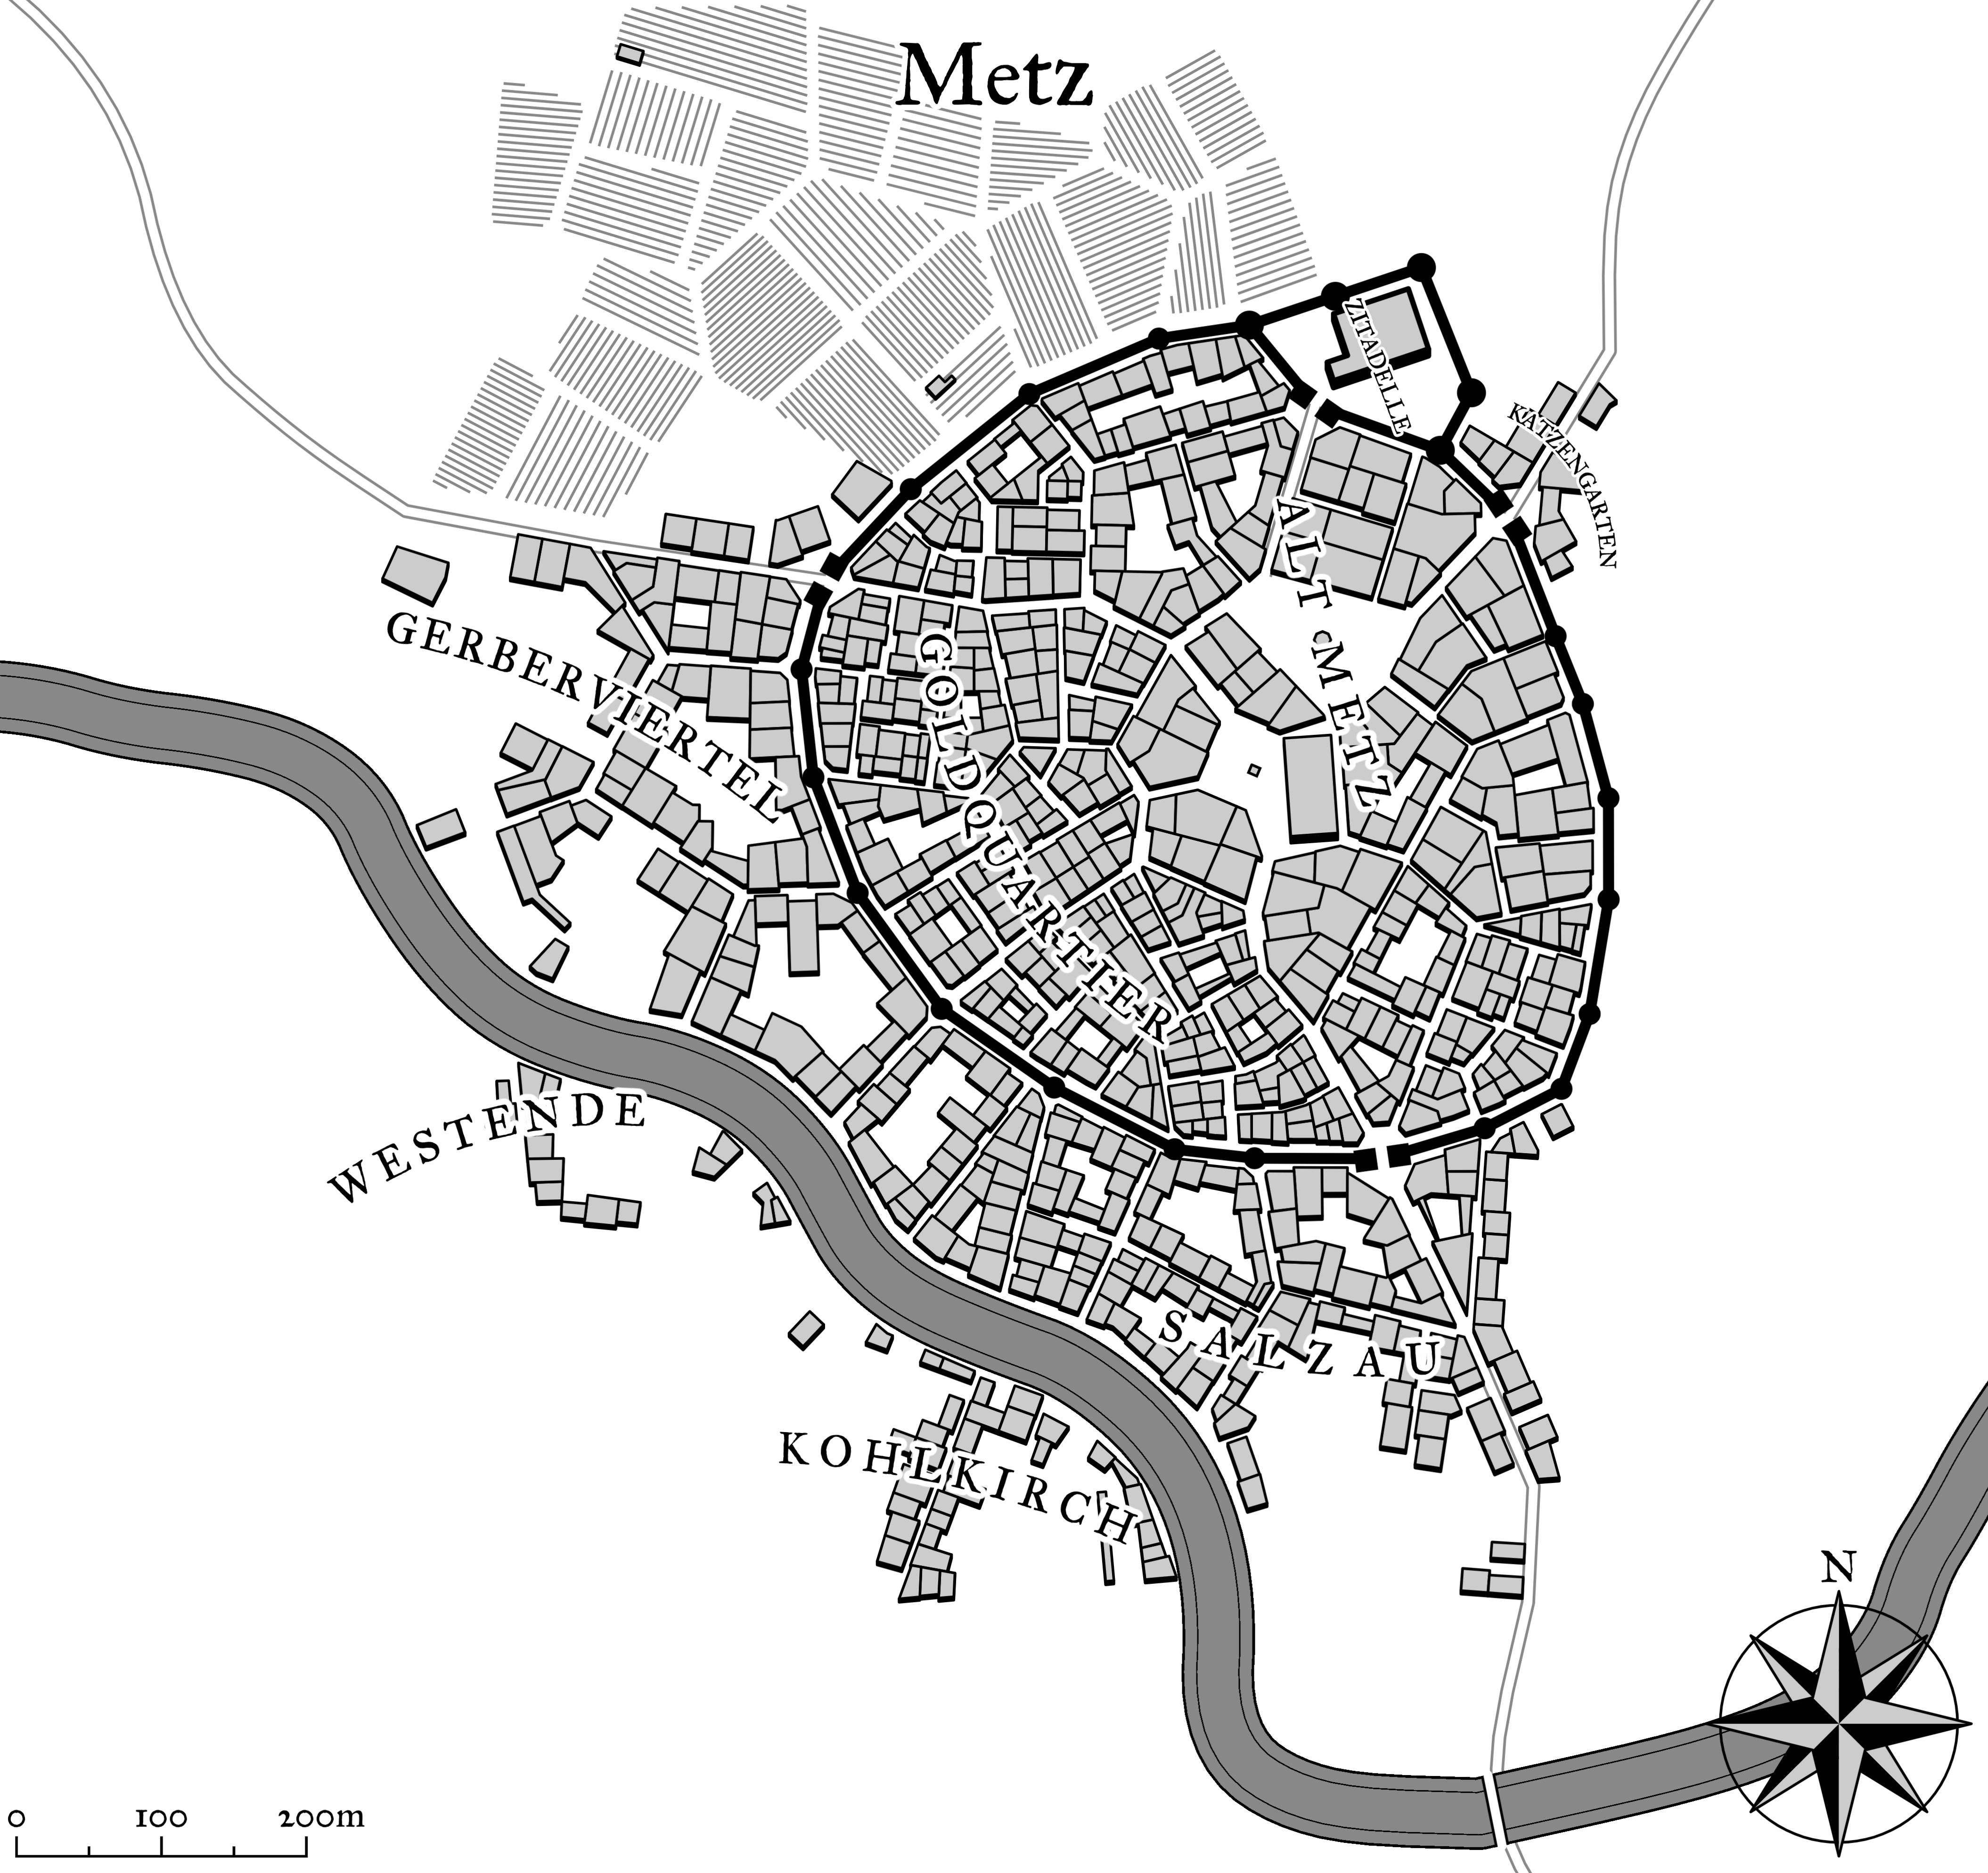
\includegraphics[width=1\linewidth]{graphics/metz} \end{center}

\section{Rumors}\label{rumors}

\begin{longtable}[]{@{}
  >{\raggedright\arraybackslash}p{(\columnwidth - 2\tabcolsep) * \real{0.5714}}
  >{\raggedright\arraybackslash}p{(\columnwidth - 2\tabcolsep) * \real{0.4286}}@{}}
\toprule\noalign{}
\begin{minipage}[b]{\linewidth}\raggedright
\textbf{1D12}
\end{minipage} & \begin{minipage}[b]{\linewidth}\raggedright
Rumor
\end{minipage} \\
\midrule\noalign{}
\endhead
\bottomrule\noalign{}
\endlastfoot
1 & Christman abducted Lise Mueller. \\
2 & Bartholomäus Bock has not been seen in a few days. \\
3 & Goetz von Berlichingen declared a feud with the city, defecated into a barrel of wine and sent it to the city council. \\
4 & Several graves have been looted in the last few weeks. Something is going on at the graveyard. \\
5 & The Gravenstein family is looking to recover an old necklace, stolen from their family crypt. \\
6 & The mayor, Sigmund Hofstatter, does not have the full backing of his council. \\
7 & The local printing press has been putting out pamphlets critical of the Church. \\
8 & Travelers have reported a group of witch hunters camping not too far away. They are looking for heretics. \\
9 & The Frassberg region in lousy with bandits. They prey just as much on each other as on travelers. \\
10 & Despite the banditry, the cloth and wine merchants have been thriving. \\
11 & Peter Stumpp, a wealthy farmer out of Bedburg, is looking for good matches for his daughters. \\
12 & The mayor is looking to hire mercenaries to deal with the bandit problem. \\
\end{longtable}

\section{What is Going On in Metz?}\label{what-is-going-on-in-metz}

\begin{itemize}
\item
  \textbf{Lise Mueller}, daughter of a respected goldsmith has vanished. The town thinks Christman took her. Regular citizens are calling for more action against the bandits. Her father, Markward Mueller, is offering an old golden torque as a reward (works like a \textbf{Ring of Protection}). He is convinced Christman took her. In reality, he only knows that Lise went for a walk along the river 2 weeks ago and never returned. If anyone asks to see her private chambers, he will be reluctant but will allow it with a strong argument. Her room has a secret compartment under the floor boards (1:6 chance). Her diary can be found there. It details how a man wreathed in shadows has been visiting her dreams and been instructing her in the ``Old Craft''. In exchange, he asked her a favor.
\item
  The \emph{Bürgermeister} of Metz, \textbf{Sigmund Hofstatter}, is keen to address the bandit problem in the region of Metz. He has big plans for more trade and sees the long-term fortune of Metz in jeopardy. He is willing to pursue a more militant strategy. He has issued a 20k gp reward for the capture of Christman, dead or alive. Furthermore, he is offering 1k gp for other bandit leaders. 10gp for a regular bandit.
\item
  A faction on the \emph{Stadtrat}, the wine and cloth merchants, have a secret agreement with Christman. They pay him handsomely to engage in his banditry away from Metz. They fear the Bürgermeister's new approach is threatening their agreement and secretly oppose him. They are scheming to have the mayor disgraced. They are considering fomenting religious strife in town with the help of the Witch Hunters. The resulting conflict might distract the mayor or even offer an opportunity to remove him.
\item
  Corpses have been vanishing from the graveyard (\textbf{Peter Niers} is using the assistant grave digger to procure fresh corpses.). Some wealthy citizens are becoming concerned and are offering a 2,000 gp reward to stop whoever is looting the graves and return a missing family heirloom (to be found in \textbf{Peter Niers'} tower).
\item
  City of Metz is in a feud with \textbf{Goetz von Berlichingen}, famous robber knight. There is a reward of 5,000 gp, financed by the guilds, for whoever can bring an end to the feud.
\item
  \textbf{Bartholomäus Bock}, local scholar and investor in the printing press, has not been seen for a few days. \textbf{Bartholomäus Bock} is a member of the Kristallbund and has a secret laboratory under his office. He recently died down there trying to create artificial life. The Kristallbund is a Secret Society, focused on the Enlightenment, magical power, and is fervently anti-religious (This is the Age of Man, not God!).
\end{itemize}

\section{The City}\label{the-city}

Metz has a population of about 16,000 people, but not all a full \emph{burgher}. The city maintains a city watch of 110 (statistics of a \textbf{Bandit}).

The city is governed by the \emph{Stadtrat}, which consists of fifteen individuals, mostly guild representatives. The \emph{Stadtrat} selects the \emph{Bürgermeister}, who has administrative authority over the city.

Main economic sectors in Metz are the trade of cloth and wine. The city also home to renowned goldsmiths and a leather working industry. Metz has two printing presses and has an emerging book printing industry.

\subsection{Alt Metz}\label{alt-metz}

\begin{itemize}
\item
  Town square and main market
\item
  Guildhall
\item
  Mayor's Hall and Court
\item
  Church of St.~Ignatius and Residence of Bishop Jean de Lorraine (86 years old, decrepit, business is run by the Vicar General)
\item
  Zum Goldvogel (inn and tavern, good quality)
\item
  Residence of wealthy citizens
\end{itemize}

\subsection{Katzengarten}\label{katzengarten}

\begin{itemize}
\item
  Vagrants, people not allowed into the city proper, and seasonal workers reside here.
\item
  Many stables are located here.
\item
  Carts and transportation can be purchased here.
\item
  \emph{Katzenjammer} tavern (poorer quality).
\item
  Note: \textbf{Peter Niers} has been using this area as his hunting grounds, kidnapping women and children. He preys on the poor, foreigners, and refugees. I avoids going after relatives of burghers, not too draw the ire of the townsfolk.
\end{itemize}

\subsection{Zitadelle}\label{zitadelle}

Headquarter of the city guard.

\subsection{Goldquartier}\label{goldquartier}

\begin{itemize}
\item
  Goldsmiths and other artisans. \textbf{Markward Mueller} has his workshop here.
\item
  Location of the office of \textbf{Bartholomäus Bock}.
\item
  \textbf{Ludolf Eggfurt} has has weapons and armor shop here.
\item
  \textbf{Anselm von Eberhart}. Alchemist and apothecary with a small shop.
\item
  Residences of well-off artisans.
\end{itemize}

\subsection{Gerberviertel}\label{gerberviertel}

\begin{itemize}
\tightlist
\item
  Tanning and leather work.
\end{itemize}

\subsection{Salz Au}\label{salz-au}

\begin{itemize}
\item
  Workers/staff and their families.
\item
  Smaller Church of St.~Augustin.
\end{itemize}

\subsection{Westende and Kohlkirch}\label{westende-and-kohlkirch}

\begin{itemize}
\item
  Poor neighborhoods on the other side of the Moselle river.
\item
  \emph{Sprungfisch Keller} (seedy tavern, hang-out for the local criminals).
\end{itemize}

\section{The Guildhall}\label{the-guildhall}

Guards: Level-2 Fighters, full plate and shield, spears and short swords or crossbow.

\textbf{1st floor}

\begin{itemize}
\item
  Main guildhall for the City of Metz. All major guilds organize their business here. During the day, citizens are welcome to enter. A clerk will receive them and ask their business. Two guards are posted outside the main entrance at all times.

  \begin{itemize}
  \item
    Clerk's hall. 2 Guards on watch during the day.
  \item
    Main meeting hall. Back of the hall has secured access to the stairs leading to the basement. 2 guards on watch during the day and night. All guildmasters have keys to access to door to the basement.
  \item
    Offices
  \item
    Servant rooms on the East side.
  \end{itemize}
\end{itemize}

\textbf{2nd floor}

\begin{itemize}
\tightlist
\item
  Guard's rooms and armory. During the day and night, 6 more guards on look-out and reserve. Alarm bell to alert the city watch of necessary.
\end{itemize}

\textbf{Secret Basement}

\begin{itemize}
\item
  Two small rooms:
\item
  3 blocked crypts with old guild masters' remains. Each can be accessed within 1 turn and appropriate tools. Karlus von Niffeling, Master of the Goldsmiths: A golden ceremonial sword worth 1,300 gp. Alois de Friis, Wine Merchant Master, 2x bejeweled ring (worth 250 gp), a potion of Poison (! not dsicernible to PCs), 1 potion of longevity. Gotfrid Hummelsberg, Cloth Merchant Master: A \textbf{Wraith}, +2 shield, +1 sword (+2 vs.~lycanthropes).
\item
  Two \textbf{Animated Armors} in the alcoves, attack anyone without a guild seal.
\item
  Main vault. Ceiling is ten feet high. Four pillars hold up the ceiling (keen eyes can spot that the ceiling can drop). Each pillar has a key hole. Four guildmaster keys have to be put here at the same time to secure the ceiling. If that does not happen within the first Turn of someone stepping into the room, a portcullis will drop and block the exit and the ceiling will descend. 2ft per round. The same mechanims also triggers an alarm bell. Niches in the walls, full of strongboxes. Each box is locked and keyed to a specific guild. Each box contains gold worth 2d6 X 1k gp.
\item
  Secret door to secondary vault. Passage with a scythe trap. Door with Wizard Lock (caster level 5). Sigil of the current Guildmaster of the cloth or wine merchants opens the door. Breaking the door causes an eldritch explosion of 4d6, save vs Breath for half. Second passage has two Rust Monsters. Second door has a puzzle lock:
\item
  Secret vault: \textbf{Lesser Efreeti} bound to protect the vault against intruders. 15k gp, 4 random MU scrolls, 2 cleric scrolls, +2 spear, 10 +1 arrows, Ring of Controlling Humans, Bag of Holding, Boots of Speed.
\item
  Document room: evidence of supplies for Christman.
\end{itemize}

\begin{center}\includegraphics[width=1\linewidth]{graphics/guild-temple-600dpi-patreon} \end{center}

\section{The Secret Workshop of Bartholomäus Bock}\label{the-secret-workshop-of-bartholomuxe4us-bock}

The House of Bartholomäus Bock has two stories.

\textbf{1st floor}
Scriptorium and office. Lockbox in the main desk (poison needle trap, 250 gp). Well-appointed library with mostly legal and religious texts. Hidden trap door to the basement and secret laboratory. Trap door is hidden under an old carpet and a chest full of writing supplies. The trapdoor is locked via \emph{Wizard Lock}.

\textbf{2nd floor}

Personal apartments. Nothing of interest here except for some gold and silver rings worth 750 gp. A portrait of Bartholomäus painted by Lucas Cranach the Elder (worth 1,200 gp).

\textbf{Basement}

\begin{itemize}
\tightlist
\item
  Each star is a construct that activates when the electricity field is turned off. Glass figures filled with swirling, multi-colored liquids and gases. When destroyed roll for effect
\end{itemize}

\begin{longtable}[]{@{}
  >{\raggedright\arraybackslash}p{(\columnwidth - 2\tabcolsep) * \real{0.4167}}
  >{\raggedright\arraybackslash}p{(\columnwidth - 2\tabcolsep) * \real{0.5833}}@{}}
\toprule\noalign{}
\begin{minipage}[b]{\linewidth}\raggedright
1D6
\end{minipage} & \begin{minipage}[b]{\linewidth}\raggedright
Effect
\end{minipage} \\
\midrule\noalign{}
\endhead
\bottomrule\noalign{}
\endlastfoot
1 & Splash damage of 1d6 acid on anyone in melee. \\
2 & Sleep spell triggered \\
3 & Caustic smoke, save vs.~Poison or spend one round coughing, unable to act. \\
4 & Paralytic agent, save vs.~Poison or half speed and you can only move or attack for 1d6 rounds \\
5 & Confusing fumes. Lose one prepared spell (determine randomly). \\
6 & Healing goo. Recover 1d6 HP. \\
\end{longtable}

\begin{itemize}
\item
  \textbf{Clockwork} (stats of a \textbf{Stone Golem}), field of electricity: once per round, a random person wearing metal armor is struck by lighting (3d6 damage, save vs.~breath for half). Determine randomly (any metal 1 chance, chain 2 chances, plate 3 chances). Fleshgolem attacks anyone trying to pass to the other side of the room.
\item
  Puddle of gore on the ground close to the Golem.
\item
  Lever all the way North can turn electricity off. Once electricity field is turned off, constructs activate and attacks anyone in the basement.
\item
  Two rooms on the right: storage. One thief trapped here.
\item
  Room on the left: personal study, spellbook (5 level 1, 4 level 2, 4 level 3, 3 level 4, 2 level 5) and scrolls (4 level 1, 4 level 2, 1 level 3, 1 level 4), Wand of Lightning Bolts, gems worth 800 gp. Coded letters indicating correspondence with other members of the Kristallbund, anti-religious activism (hooks for other adventures can be inserted here).
\end{itemize}

\begin{center}\includegraphics[width=1\linewidth]{graphics/golem-crypt-of-ul-vir-the-mad-patreon-grid} \end{center}

\chapter{Bedburg}\label{bedburg}

\begin{center}\includegraphics[width=1\linewidth]{graphics/bedburg} \end{center}

Small farming community. 130 souls.

\section{Rumors}\label{rumors-1}

\begin{longtable}[]{@{}
  >{\raggedright\arraybackslash}p{(\columnwidth - 2\tabcolsep) * \real{0.5714}}
  >{\raggedright\arraybackslash}p{(\columnwidth - 2\tabcolsep) * \real{0.4286}}@{}}
\toprule\noalign{}
\begin{minipage}[b]{\linewidth}\raggedright
\textbf{1D8}
\end{minipage} & \begin{minipage}[b]{\linewidth}\raggedright
Rumor
\end{minipage} \\
\midrule\noalign{}
\endhead
\bottomrule\noalign{}
\endlastfoot
1 & Rumors about strange happening at the Stumpp farm. \\
2 & Rumors about bandits being behind the attacks. \\
3 & Wolfs have been sighted in the area. \\
4 & Peter Stumpp is trying to marry off one of his daughters to a merchant from Metz. \\
5 & A local wants the Witch Hunter to come. \\
6 & Stumpp is the wealthiest farmer. \\
7 & He is looking to marry off his daughters and is entertaining proposals. \\
8 & Frieda Meier has vanished (abducted by Peter Niers). 3 months ago Karla Boxberg did not return from a trip to Metz. \\
\end{longtable}

\section{What is Going On?}\label{what-is-going-on}

\begin{itemize}
\tightlist
\item
  String of grisly murders.
\item
  Peter Stumpp, wealthy farmer, is afflicted by a curse. Has begun to lock himself into his barn every night.
\item
  Hags in Hex 0200 have cursed Peter as punishment for a slight (denied them his daughter).
\item
  The town council is willing to pay 500 gp for solving the wolf attack problem. Local loggers have been attacked.
\item
  If staying in Bedburg, random chance of a werewolf attack at night, depending on moon phase.
\end{itemize}

\section{Peter Stumpps' Farm}\label{farm}

\begin{center}\includegraphics[width=1\linewidth]{graphics/tarsakh-manor-ground-floor} \end{center}

\begin{itemize}
\item
  Stumpp farm is a bit outside of town.
\item
  At the farm, Peter Stumpp lives with his four daughters (Maria 21, Evelyn 18, Rosalie 15, Trine 12) and 6 farm hands and 3 maids. Maria is to be betrothed to a wine merchant from Metz, solidifying a business alliance. Stumpp has ownership over hills suitable for wine production. He is also entertaining proposals for his Evelyn.
\item
  Peter Stumpp has been cursed by the hags (he thinks they are witches) and is trying to protect his family and innocent bystanders from his attacks. He will lock himself into his barn at night.
\item
  Visiting his farm, the barn has been visibly reinforced. The windows are boarded up and the door is steel reinforced. Inside: chains attached to a central post.
\item
  Peter Stumpp has a 1-8 chance of transforming into a werewolf every night. When the moon is full, the chance rises to 5-6. After 13 transformations, he will embrace his new nature as a werewolf and turn Neutral Evil, hunting humans for sport.
\item
  Wolf packs in the region follow his commands and will respond to his emotions. When he transforms, the wolfs become very aggressive as well and attack humans.
\item
  Can Peter Stumpp be cured? Yes, a Cleric can lift the curse as long as Peter Stumpp still resists the transformation. The hags can also be convinced to lift the curse in exchange for one of his daughters.
\item
  Peter Stumpp has hidden in his farm a treasure chest with 3,000 gp and a magical axe +2 (with an exploding damage die).
\end{itemize}

\chapter{Waldrach}\label{waldrach}

\begin{center}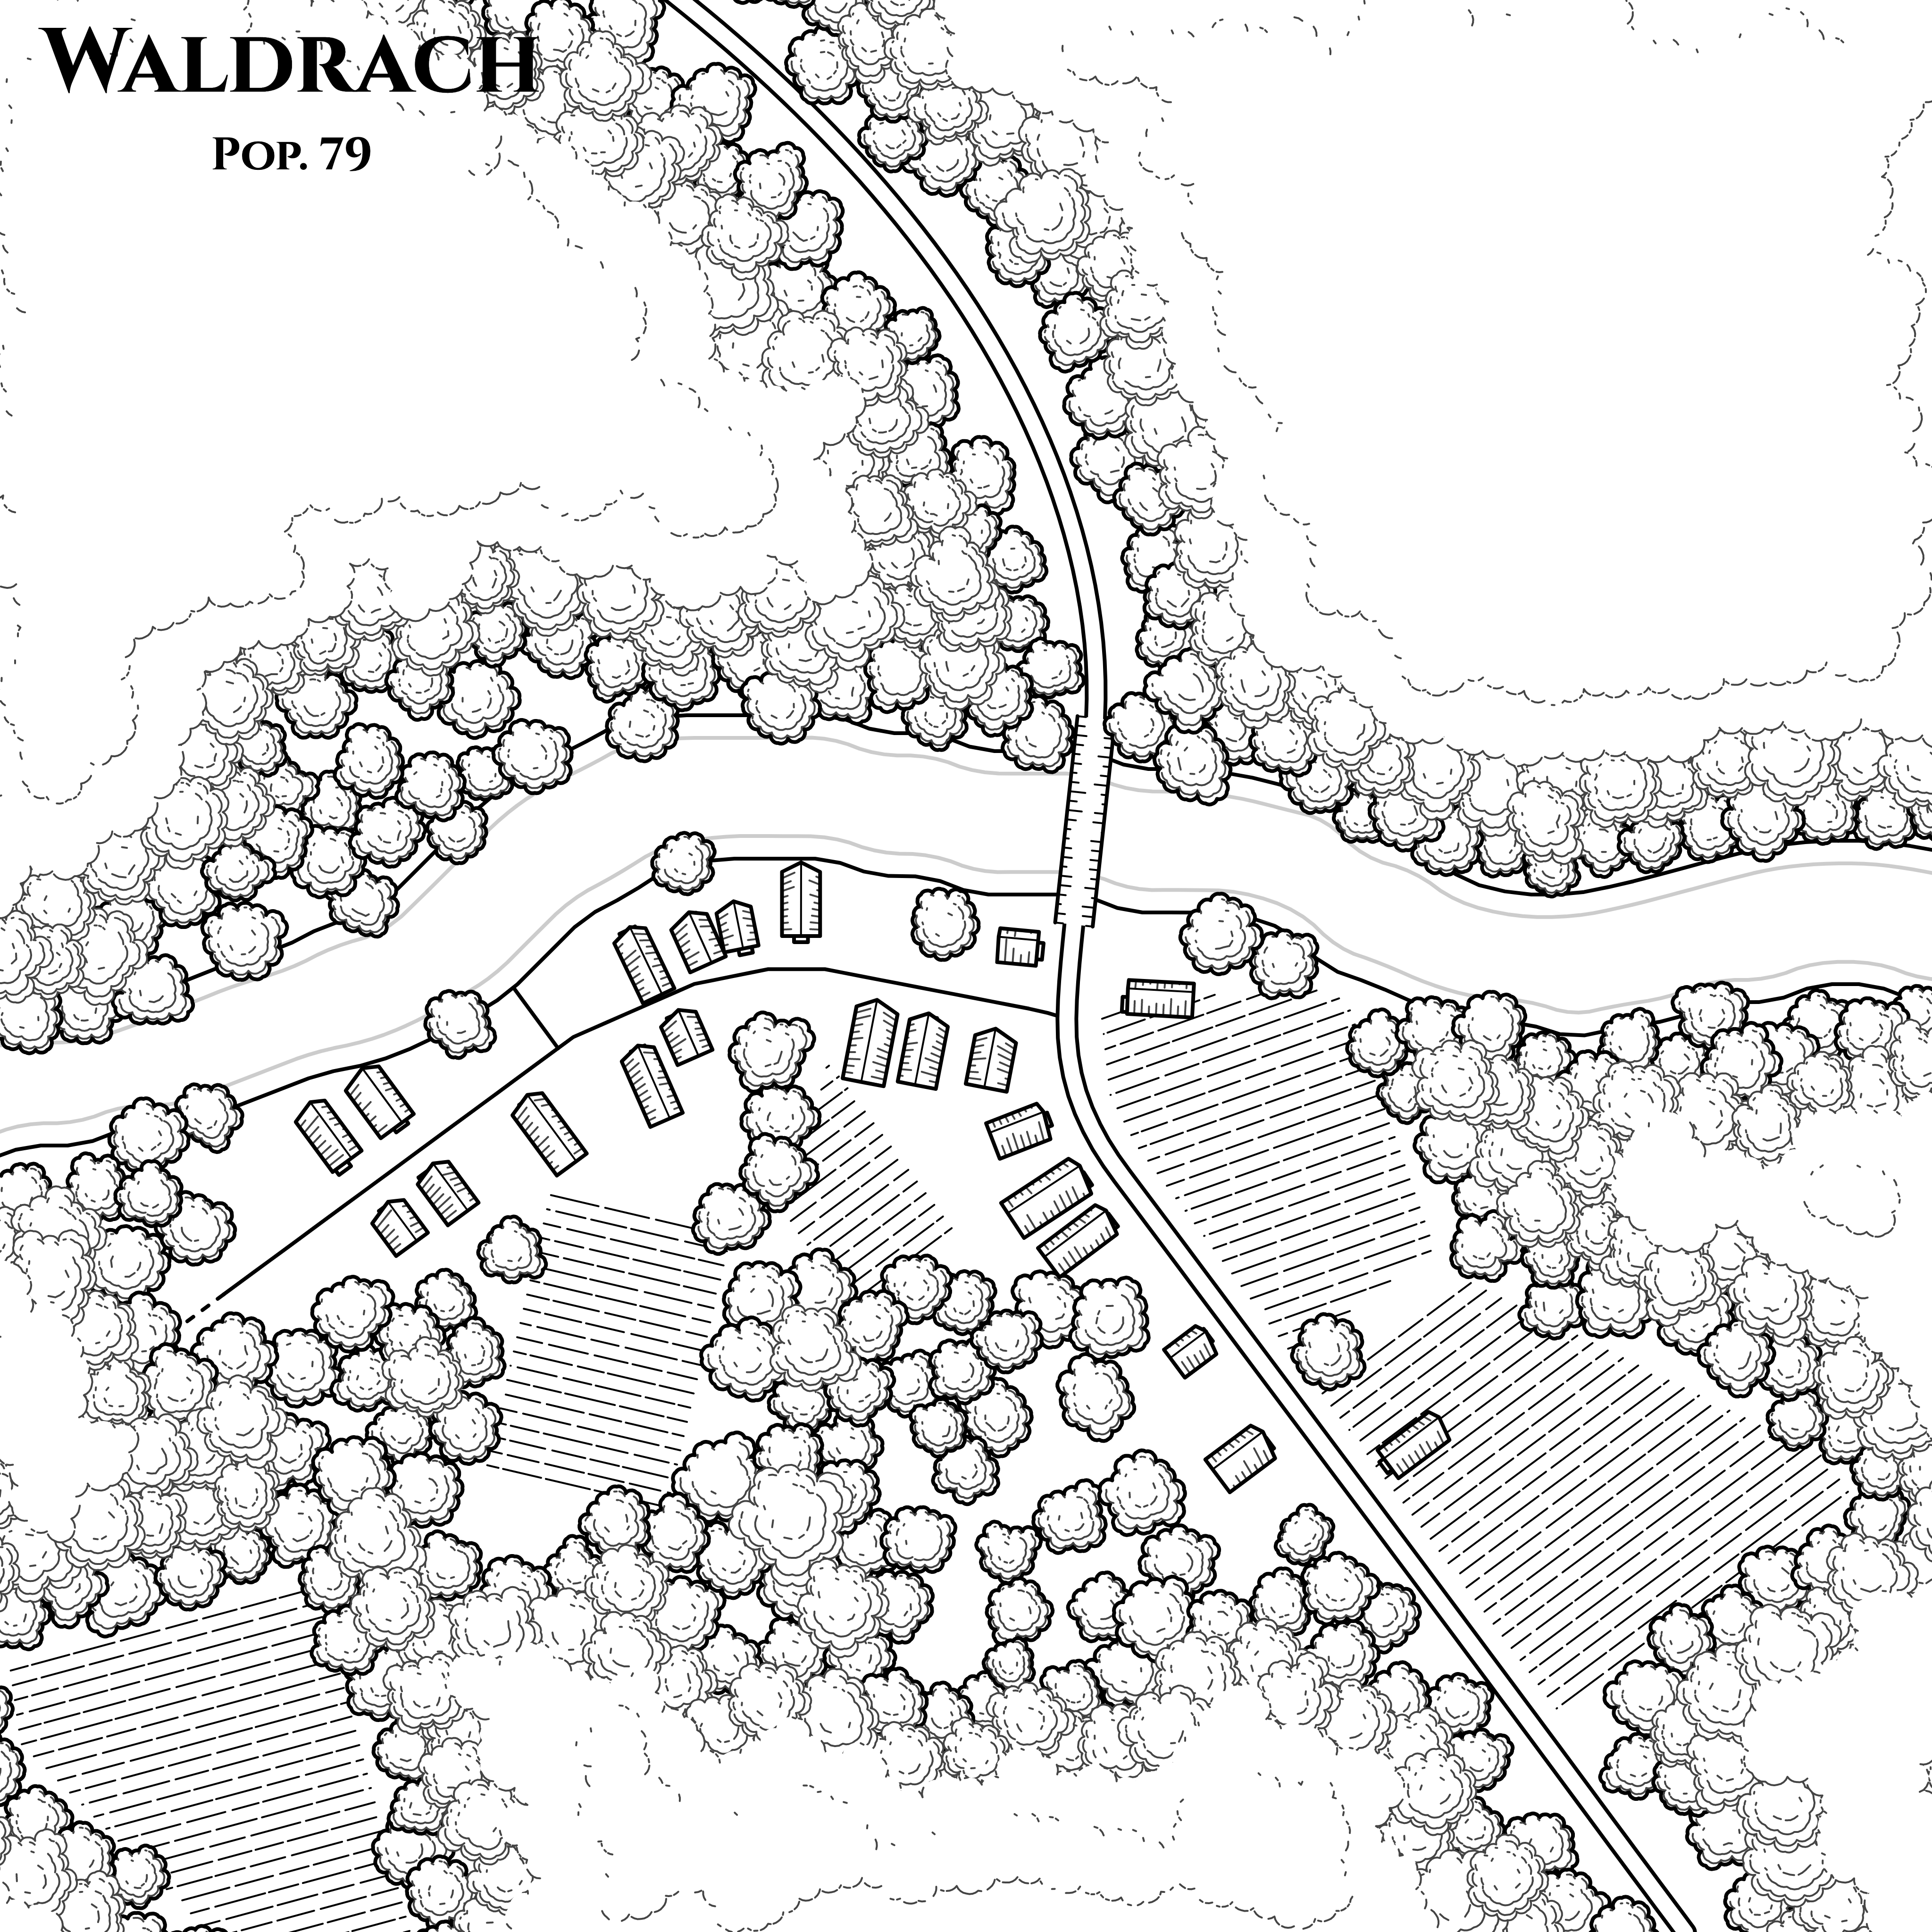
\includegraphics[width=1\linewidth]{graphics/waldrach} \end{center}

\section{Rumors}\label{rumors-2}

The locals are nearly all on the side of the Waldrach Clan and won't let much slip. In the Waldrach Brewery, traveling guests will share rumors freely. Roll on the general rumor table.

\section{What is Going On?}\label{what-is-going-on-1}

\begin{itemize}
\item
  Town is in league with Christman
\item
  Local brewery supplies him with beer, ale, and wine
\item
  Have also damned up the river, screwing a mill downriver.
\item
  Regular but secret transports of supplies and coin for Christman from the merchants of Metz. One driver and one disguised guard on the way to Waldrach from Metz. Handover in Waldrach, from there the Waldrach family handles business and carries supplies to the Frassberg once a month (on the 3rd of each month).
\item
  The town is mostly the large brewery/tavern/guesthouse and the clan members' homes.
\item
  There is a small parish church. \textbf{Father Ignaz} is the local priest. He is very young and inexperienced. Knows some of the affairs of the Waldrach Clan and disapproves but was seduced by one of the Waldrach girls. Klaus Waldrach is threatening to reveal the secret to the Church. He is trying to find a way out of his dilemma.
\item
  Klaus Waldrach's son, \textbf{Berthold}, is brash, arrogant, and a braggart. Can be found holding court at the brewery. He is pushing the takeover of the mill. Will pay adventurers 1,000gp to make the miller sell or leave. Klaus is letting Berthold pursue this to test his son.
\item
  Klau's brother, \textbf{Otto} (Thief-4) is his quiet, second-in-command. He is in charge of the supply runs to Christman.
\end{itemize}

\section{The Waldrach Brewery}\label{the-waldrach-brewery}

\begin{itemize}
\item
  Waldrach clan has 27 members in town (stats of an \textbf{Berserker}, varied weapons.)
\item
  Plenty of treasure and magic items in the basement.
\item
  Strange collection of NPC guests
\end{itemize}

\begin{longtable}[]{@{}
  >{\raggedright\arraybackslash}p{(\columnwidth - 2\tabcolsep) * \real{0.4348}}
  >{\raggedright\arraybackslash}p{(\columnwidth - 2\tabcolsep) * \real{0.5652}}@{}}
\toprule\noalign{}
\begin{minipage}[b]{\linewidth}\raggedright
\textbf{1D20}
\end{minipage} & \begin{minipage}[b]{\linewidth}\raggedright
RANDOM GUEST
\end{minipage} \\
\midrule\noalign{}
\endhead
\bottomrule\noalign{}
\endlastfoot
1 & 3 young nobles traveling \\
2 & 1d4 monks on the way to Würzburg \\
3 & Lady Liesenburg and her daughter Amalia on the way to Nordhausen to visit her sister. \\
4 & Carpenter apprentice on the Walz \\
5 & Merchant with porters and 1 guard \\
6 & 1d4+1 Mercenaries looking for employment \\
7 & A dwarf clockmaker, Conrad Baumgartner, on the way to Bruckstadt \\
8 & Fernando Ortiz, M-U (Level 4) \\
9 & 1d4 Members of Wilhelm von Hagen's camp, looking for information about heretics \\
10 & Cloth merchant from Metz (complaining about a recent lost shipment.) \\
11 & Traveling bard \\
12 & Locals (will gossip about the Waldrach Clan if sufficiently drunk). \\
13 & A Turkish Mathematician. Willing to sell a copy of his most recent manuscript for 200 gp. 6 hrs of study and a successful Int check reveals a random L2 MU spell. \\
14 & Postman \\
15 & Farmer \\
16 & Teacher \\
17 & Student \\
18 & Craftsman \\
19 & Priest \\
20 & Stagecoach driver \\
\end{longtable}

\begin{center}\includegraphics[width=1\linewidth]{graphics/brewery-ground-floor} \end{center}

\begin{center}\includegraphics[width=1\linewidth]{graphics/brewery-second-floor} \end{center}

\begin{center}\includegraphics[width=1\linewidth]{graphics/brewery} \end{center}

\begin{center}\includegraphics[width=1\linewidth]{graphics/brewery-basement} \end{center}

Guest rooms are in other nearby buildings.

1st floor: brewery and alehouse

2nd floor: Alehouse

3rd floor: Waldrach clan rooms.

Basement: Kegs, barrels, brewery supplies, locked vault with weapons and treasure (3,327 gp), secret tunnel leading closer to the Frassberg, used to bring supplies to Christman (terminates in \textbf{Hex 0402}.). The stored ale is worth 12,500 gp (many barrels). 2x Potion of Giant Strength.

\chapter{Peter Niers' Tower}\label{tower}

\begin{center}\includegraphics[width=1\linewidth]{graphics/guimonds-tower-and-druid-lich-lair-patreon annotated} \end{center}

\section{Background}\label{background}

Peter Niers stumbled on this old wizard's tower two years ago and has made it his lair. He has been scheming from the tower to wrestle control of the different bandit groups from Christman and terrorize the wider region.

He is slowly building his retinue of undead by attracting them from the local area and paying the grave digger of Metz to deliver him 4 more bodies every week.

When Peter Niers has amassed 33 undead and struck a deal with the \textbf{Greencloak Pikes}, he will attack Christman's Lair to claim the \textbf{The Rites of the Pale Wedding}.

\section{Wandering Monsters}\label{wandering-monsters}

\begin{longtable}[]{@{}ll@{}}
\caption{Encounter Table Tower}\tabularnewline
\toprule\noalign{}
\textbf{1D100} & \textbf{Encounter} \\
\midrule\noalign{}
\endfirsthead
\toprule\noalign{}
\textbf{1D100} & \textbf{Encounter} \\
\midrule\noalign{}
\endhead
\bottomrule\noalign{}
\endlastfoot
1--20 & 1D6+4 Zombies. Undead Landsknechte. \\
21--40 & 2D12 Skeletons \\
41--50 & 1D6 Ghouls \\
51--55 & 1 Ghast and 1D6+2 Ghouls \\
56--60 & 1D6 Wights. \\
61--65 & 1D4 Wraiths. \\
66--75 & 1 Ghost \\
76--80 & 1 Revenant \\
81--85 & 1D3 Spawn of the Worm \\
86--100 & Peter Niers. \\
\end{longtable}

Peter Niers is always accompanied by 2 \textbf{Wraiths}.

\section{The Tower}\label{the-tower}

No birds or insects within 50ft of the tower. Just sticky air and an oppressive silence.

\textbf{Area 1}
Wooden shed built adjacent to the tower. Main entrance. Simple wooden door (locked). Inside the shed, bits and pieces of human bodies. A \textbf{Carrion Crawler} hides on a hole under the stone steps. Simple stone steps to the tower entrance.

\textbf{Area 2}
Reinforced wooden door (locked) and covered in arcane symbols (\emph{Alarm} spell). South wall a treasure chest with a poisoned dart (Save vs poison or death). Chest contains alchemical ingredients, 2 level 3 MU spell scrolls, the lost necklace of the Gravenstein family (3500 gp), 650 gp). Two doors on the Western side (unlocked). Both doors are covered in frost. A set of stairs in the North leading up to level 2.

\textbf{Area 3}
Storage room. Peter Niers cast a cold spell on the whole room. Filled with 12 corpses and individual body parts.

\textbf{Area 4}
Secret trapdoor to the basement area--Peter Niers' actual hideout. Covered with dirt and sand. The other sides of the tower have grass growing.

\textbf{Area 5}
Level 2 of the tower. Southwestern wall has collapsed. Spiraling staircase on the Western side. Empty.

\textbf{Area 6}
Western and Eastern Walls have collapsed. 6 \textbf{Skeletons} with spears hold guard. Will push intruders off the tower (30ft drop. Save vs breath or take 2d6 damage.)

\textbf{Area 7}
Top floor of the tower. Arcane summoning circle in the middle. This is were Peter Niers converses with the devil \textbf{Zalfaxx}, which he summoned weeks ago. \textbf{Zalfaxx} told Peter Niers about the \textbf{Bone Idol}.

A \textbf{Bone Golem} stands guard.

\textbf{Zalfaxx} is willing to parlay with intruders and betray Niers, e.g., tell them about his \textbf{Bone Idol} and that the \textbf{Remains of St.~Jakobus} can counteract it.

\textbf{Area 8}
Entrance to the basement. Wet and slippery stairs lead down into a crumbling basement.

\textbf{Area 9}

\textbf{Area 10}
Square room with a large central pillar (tower foundation). Scorch marks on the stones. Northern wall with 5 niches. Each niche has a grave candle. Candles 2, 3, 5 are lit. Extinguishing all candles reveals the secret tunnels on the Eastern side. Lighting all candles triggers a fireball spell.

Two tunnels on the Eastern side that lead deeper underground into a natural cave. Hidden by illusion magic.

\textbf{Area 11}
Central cave with a dark pond, 10ft deep. A \textbf{Gibbering Mouther} nests here and protects Peter Niers' hideout.

\textbf{Area 12}
Peter Niers' camp. A bedroll, candles, rations, his spellbook. He keeps a rotting corpse here to fall asleep next to.

\textbf{Area 13}
Small altar were Peter Niers keeps the \textbf{Bone Idol}. The Idol was empowered through human sacrifice. Implied evidence for the sacrifice of fetuses.

\textbf{Bone Idol}. Permanent effect of the \emph{Carrion Stench} spell. Slowly raises and attracts up to 33 undead in a 24 mile radius. Brandishing the \textbf{Bone Idol}, the owner can command the undead. For the purposes of turning undead in the presence of the \textbf{Bone Idol}, treat the cleric as one level lower.

\textbf{Rites of the Pale Wedding}. A dark ritual to attain lichdom. The ritual requires a body assembled from human flesh, the sacrifice of several human lives, and a ritual incantation under the pale moon, completing a wedding ritual. Upon completion, the caster is turned into a lich. The caster transfers their soul into the body of the dead bride. Completing the wedding vows raises the bride to undeath and turns her into a walking phylactery. Peter Niers believes this is a way to achieve lichdem and creating a wife that will fulfill his every whim.

\textbf{The Truth}. The Ritual is a trap. Completing the ritual does make the caster a lich, but not in the way typically imagined. Transferring a piece of your soul to the undead bride fills her with unlife, giving her a full and independent (malignant) personality, with a deep loathing of the caster. The transfer also renders the caster unable to ever cast spells again. The bride in turns becomes a M-U of the same level as the ritual caster and knows all the caster's spells. The caster gains eternal unlife, but is bound to be a rotting wretch, tied to the bride in eternal servitude. The caste retains their spell slots, which the bride can use at will to power her own spells, as long as the caster is within 30ft of the bride. The caster essentially becomes a spell battery. The Ritual can be easily adapted to switch or change the genders of the caster or bride

\chapter{Christman's Lair}\label{lair}

\section{General Notes}\label{general-notes}

ADD TIMETABLE FOR CHRISTMAN?

This is Christman's secret lair in the Frassberg region. He has lived here for decades and made the cave system his home. There are three ``factions'' active in the dungeon:

\begin{itemize}
\item
  \textbf{Christman Grippertenius}. Spends most of his days drinking himself into a stupor. Will either kill or capture any intruders. Prisoners will be tortured and eventually killed. He treats Lise Mueller as a scullery maid and otherwise ignores her. He is afraid of the ghost of Getrude Kaasman. If he thinks a part of the cave system is currently being haunted by the ghost, he will move as far away as possible.
\item
  \textbf{Lise (Lischen) Mueller}. A satanic witch. She let herself be captured by Christman and is his current ``wife''. Christman is known for haven taken many ``wives'' (i.e., abducted women and kept them in his dungeon against their will) over the years. In his old age, he has done so less frequently and mostly does it out of habit and for having someone around to help him clean. Lise is a cunning witch that has out herself into Christman's hands in order to conceive a child with him. Because Christman has no interest in her (or anyone for that matter) and is mostly drunk, she is scheming to spoil is alcohol supply, cut off future deliveries, and otherwise get him to pay attention to her. She is not beyond considering murdering Christman to get what she needs from his corpse. She has cast Charm on Christman, but his black soul has weakened the effects of the spell. Deep down, Christman fears Lise and tries to find excuses to be away from her.
\item
  The ghost of \textbf{Gertrude Kaasmann}. One of Christman's prior ``wives''. He murdered her and her child 23 years ago. She is a mere echo of a mother's grief and a general menace to any living creature. If she can be made to remember what happened to her, she can become an, albeit temporary, ally against Christman.
\end{itemize}

There are otherwise few creatures about in the dungeon. Christman's lair is a murderhole which he stalks like a predator. Try to play up the atmosphere of discovering serial killer's home (e.g., think Jame Gumb's basement in the movie Silence of the Lambs).

Christman has accumulated a huge amount of treasure over the years. Anyone brave enough to enter the caves and survive, might lay claim to unimaginable riches.

Due to Christman's familiarity with the dungeon, the base chance of Surprise increases from 2-6 to 4-6 for PCs. If Christman retreats from a fight, he has a 2-6 chance of simply vanishing when he runs into another room and PCs lose line of sight. This is not a supernatural ability and if PCs have extraordinary means of keeping track of Christman, this ability is countered.

\section{Level 1}\label{level-1}

\begin{center}\includegraphics[width=1\linewidth]{graphics/shut-your-gobhole annotated} \end{center}

\textbf{Wandering Monsters}

\begin{longtable}[]{@{}
  >{\raggedright\arraybackslash}p{(\columnwidth - 2\tabcolsep) * \real{0.3913}}
  >{\raggedright\arraybackslash}p{(\columnwidth - 2\tabcolsep) * \real{0.6087}}@{}}
\caption{Encounter Table Christman's Lair}\tabularnewline
\toprule\noalign{}
\begin{minipage}[b]{\linewidth}\raggedright
\textbf{1D100}
\end{minipage} & \begin{minipage}[b]{\linewidth}\raggedright
\textbf{Encounter}
\end{minipage} \\
\midrule\noalign{}
\endfirsthead
\toprule\noalign{}
\begin{minipage}[b]{\linewidth}\raggedright
\textbf{1D100}
\end{minipage} & \begin{minipage}[b]{\linewidth}\raggedright
\textbf{Encounter}
\end{minipage} \\
\midrule\noalign{}
\endhead
\bottomrule\noalign{}
\endlastfoot
1--45 & 1D6+3 of (18 total) Christman's Dogs. All teeth and mangy fur, ribs showing. Beaten but loyal. \\
46--65 & Lise Mueller. \\
66--80 & Alcoholic Ooze. \\
81--85 & The ghost of Getrude Kaasmann. \\
86--100 & Christman (1-4 drunk, 5-6 sober). \\
\end{longtable}

\textbf{L1}: Main entrance to the cave. Smells of acrid smoke. Graffiti on the wall at the entrance: ``Cristman's Castle''. 6ft further down the tunnel, PCs can see more markings on the wall. The markings are pure gibberish, trying to invoke a foreign alphabet. Christman built a spiked pit trap (8ft deep) filled with lye right next to the markings. Save vs breath (DCC: Reflex save DC 10) or take 1d6 damage from the spikes and 1 point of caustic burn damage for every round in the pit. If the PC took 4 or more points of damage from the spike, they injured one of their extremities and it is more difficult to climb out of the pit.

\textbf{L2}: Secret entrance on ground level, completely covered by poison ivy. Touching the ivy Save vs Poison (DCC: Fort save DC 11) or develop a serious rash that lingers for 1d4 days. Cannot wear armor while afflicted by the rash. Cure Disease (DCC: Lay on Hands for 2 HD) removes.

\textbf{L3}: Secret entrance. On a ledge 20ft up from the ground and hard to see. At the cave entrance, a thin tripwire is connected to a bell to the alarm bells in L4. When bells are rung, 1D6+3 of Christman's dogs appear within 1 turn.

\textbf{L4}: Central intersection. Tripwires with alarm bells. Bells attract 1D6+3 of Christman's dogs appear within 1 turn.

\textbf{L5}: Room with a barricade that faces and blocks access to L4. An additiona piece of barricade can be moved quickly to block the northern exit. Two loaded crossbows lean against the wall. They have poisoned arrow tips. If hurt, save vs Poison (DCC: Fort save DC 12) or spend 1d3 rounds wretching and unable to act.

\textbf{L6}: Kennel room. Smells like dog feces and urine. Barks can be heard when approaching. 6 dog kennels total, only one is closed. Inside, one injured but aggressive dog (sprained leg). One large kennel is up on the elevated rock ledge. Old carpets and furs on the ground. They cover a hidden pressure plate. If someone steps on it, spring-loaded wooden barriers block the two exits and the door to the kennel on the elevated rock ledge opens.Inside this cage is a hungry \textbf{Bear}, trained by Christman to prefer human flesh.

\textbf{L7}: The smell of dog urine and feces. The room is filled with additional dog kennels. Barrels full of dog food. There are at least 1d6+2 dogs resting in this room.

\textbf{L8}: Storage room. Filled with sacks of flour, barrels of fish, cheeses, smoked meats. Cage with iron bars and a heavy lock (DCC Pick locks DC 7). Inside are racks of wine (60 bottles of wine, each worth 20 sp). At the Northwestern side of the room, a wall carpet hides a secret vertical, winding tunnel with a rope that leads to Level 2 (\textbf{L24}).

\textbf{L9}: Fletchery. Chaotic workshop, tools strewn about, pieces of wood, piles of feathers. Whoever is working here has high skill, but is extremely untidy and disorganized. A total of 37 arrows can be recovered from this room. Northern side has a tunnel exit that leads to Level 2 (\textbf{L14}).

\textbf{L10}: From the ceiling hang long wires with thin glass bulbs attached. The lenght of the wires varies from 1 ft off the floor to 5ft off the floor. The bulbs do not touch each other and there is at most 1 ft room between two bulbs. There are burns marks all over the floor and walls. The glass bulbs are filled with a highly-reactive alchemical substance that is activated when moved about too much. If someone carelessly walks through the room and a bulb starts swinging, it triggers a reaction and the bulb explodes in a fiery explosion, sending glass shards everywhere. This triggers all other bulbs to explode. Carefully traversing the room requires a Save vs.~Breath (DCC Reflex save DC 12) (or some other approach). Failure triggers the trap and causes 6d6 explosion damage to anyone in the room and 2d4 continued alchemical burn damage for 1d4+2 rounds (the goey substance does not come off easily).

\textbf{L11}: A terrible smell of decay, feces, and urine. A room used for skinning and tanning room. Several skinned animal carcasses hang from the ceiling (some have human bite marks). One skinned human carcass among the animals. A trough for tanning.

Hanging like wind chimes from the ceiling, dried, stretched out and flayed baby corpses.

``Tanzt liebe Kindlein tanzt, Gnipperteinga euer Vater macht euch den Tanz''

\textbf{L12}: A storage room. Nine large wooden and closed barrels. Barrels contain human bodies in a brine solution.

\textbf{L13}: Storage for discarded clothes, arms, armor from killed enemies (3 sets of leather armor, 1 set of chain mail, 3 spears, 2 bows, 1 long sword, 2 short swords). Three cave wasp nest on the ceiling, one more nest build into a set of magical +1 plate armor. Wasps will react to any disturbance in the room.

\section{Level 2}\label{level-2}

\begin{center}\includegraphics[width=1\linewidth]{graphics/twilight-descent annotated} \end{center}

\section{Wandering Monsters}\label{wandering-monsters-1}

\begin{longtable}[]{@{}
  >{\raggedright\arraybackslash}p{(\columnwidth - 2\tabcolsep) * \real{0.3913}}
  >{\raggedright\arraybackslash}p{(\columnwidth - 2\tabcolsep) * \real{0.6087}}@{}}
\caption{Encounter Table Christman's Lair}\tabularnewline
\toprule\noalign{}
\begin{minipage}[b]{\linewidth}\raggedright
\textbf{1D100}
\end{minipage} & \begin{minipage}[b]{\linewidth}\raggedright
\textbf{Encounter}
\end{minipage} \\
\midrule\noalign{}
\endfirsthead
\toprule\noalign{}
\begin{minipage}[b]{\linewidth}\raggedright
\textbf{1D100}
\end{minipage} & \begin{minipage}[b]{\linewidth}\raggedright
\textbf{Encounter}
\end{minipage} \\
\midrule\noalign{}
\endhead
\bottomrule\noalign{}
\endlastfoot
1--25 & 1D6+3 of (15 total) Christman's Dogs. All teeth and mangy fur, ribs showing. Beaten but loyal. \\
26--50 & Lise Mueller. \\
51--70 & Alcoholic Ooze. \\
71--80 & Gustavo Pellegrini. \\
81--100 & Christman (1-4 drunk, 5-6 sober). \\
\end{longtable}

\textbf{L14}: Stone platform. South: Stairs descending from Level 1 \textbf{L9}. Northeast: Winding, roughly-hewn stone steps that lead down to \textbf{L15}. No railing, the uneven steps make it easy to tumble off. If running down the steps, \textbf{Wand Save} (\textbf{DCC: Reflex Save DC 8}) or take 1d6 bludegeoning damage from falling on hard stone. North: Stone steps that are cut from the stone wall, leading upward at a slight incline. Wooden doors (unlocked) that lead to \textbf{L29} and \textbf{L18}. Southwest: Locked wooden door (\textbf{DCC: Pick locks DC 6 or STR check DC 9}) to \textbf{L30}.

\textbf{L15}: Central treasure room. Barrels of acid hanging on the ceiling, held by a complex rope and pulley system. If Christman is here, he can use the many ropes and pulleys to trigger a acid barrel splash attack: Save vs Breath (\textbf{DCC: Reflex Save DC 12}) or take 3d6 acid damage, half if saved successfully. \textbf{Treasure}: This is Christman's main hoard. Uncaringly thrown on the ground, 623 gp (there is an oily, translucent film on the coins--contact poison; Save vs Death / \textbf{DCC Fortitude save DC 15}; failure means death, success 2d6 damage, loss of 2 points of Constitution/Stamina and incapacitated for 1d2 turns), 23,440 sp, 8,103 cp, jewelry worth 1,900 sp, gems worth 3,600 sp, magic items. Treasure sits on weighted plates that trigger a bell and an acid splash (the bell attracts the dogs and Christman).

\textbf{L16}: Grave niches. Two empty, roughly dug grave niches, filled with trash (clothing, spoiled food, 27 sp under some rags). Two niches are filled with wooden coffins. Carved on the northern coffin: \emph{Maria}, Southern coffin: \emph{Rabea}. Christman buried two of is former ``wives'' here. If opened, the northern coffin contains a skeleton and a beautiful gold necklace worth 1,000sp. The other, a decomposing corpse (maybe 2 months old) full of worms and 1d4 \textbf{Rotgrubs} that attack anybody who searches the body. The insides of the coffin show scratch marks and a fingernail stuck in the wood. On the bloated corpse, a simple wooden cross with a carved depiction of Jesus (if returned to the camp of \textbf{Alois Hutmeister}, the PC receive a reward of 3 healing potions. Rabea was a well-liked camp cook that vanished four months ago).

\textbf{L17}: Gustavo's prison. Heavy wooden door, reinforced with steel. Faint sounds of humming from the other side. Unlocked but closed. Christman is carrying one key. Another key can be found in \textbf{L26}. Inside, a dirty and malnourished \textbf{Gustavo Pellegrini}. He is a traveling minstrel that was captured by Christman while wandering too close to the lair. He spends most of his time in the cell, but sometimes, he roams around. After a prolonged period of torture, Gustavo believes Christman is the devil and he is unable to leave on his own account. Will betray the PCs to gain favor with Christman (e.g., lure them into a trap or bring them to Christman).

\textbf{L18}: Flaying room. Stone slab in the middle of the room, coated in dark, red blood. Four wooden frames with human skin spun across. To the north, a small room with tools (knifes, knife sharpener, saws, etc.). Lise has been painting satanic runes on the skins. MAGICAL TRAP.

\textbf{L19}: Ice box. Locked door, cold to the touch. Inside, a large shard of ice, protruding through the stone floor (related to the Ice Giant's presence at the Frassberg peak). The floor is slippery. Breath save/Reflex save DC 8 to not fall when attacking in combat (unless precautions are taken). Magical, exuding harsh cold. Souther niche is storage for human bodies and animal meat. Northern niche side of the room is covered in partially opaque ice. Under the ice, barely visible, two dead bodies holding a sword. The sword is magical, the two bodies are \textbf{Wights} that attack if cut out of the ice.

\textbf{L20}: Lise's painting studio. A single, wooden frame with a human skin. Paints and brushes, a chair.

\textbf{L21}: Cool cave. Storage for food, liquor, ale, and wine. Smoked ham, sausages, sacks of flour and oats, honey, sugar, butter, 23 bottles of fine wine (worth 40 sp each), 10 barrels of ale (worth 50 sp each), 40 bottles of Schnaps (worth 15 sp each). Stone stairs lead up to \textbf{L39}.

\textbf{L22}: Empty cross walk. One of the side niches contains a skeleton with a leather belt and a fine leather seath. Inside, a \emph{+1 dagger}.

\textbf{L23}: Several Persian rugs cover the stone floor (5 rugs total, each worth 250 gp but heavy and bulky). Eight stuffed heads of Christman's enemies decorate the walls. The heads are all defaced (e.g., eyes sown shut, animal parts sown on, genitalia stuffed into the mouth). One of the rugs covers a spiked pit trap: \textbf{Save vs Breath} (DCC: Reflex Save DC 12) or 3d6 damage.

\textbf{L24}: Empty hallway. In the Northern end, rope affixed with iron pitons that leads through a winding tunnel up to \textbf{L8}.

\textbf{L25}: Walls, floor, and ceiling are covered with rough charcoal sketches of people, faces, and murder scenes. Christman has drawn all his murders here and comes to the room to relive the experience, while pleasuring himself. The room is filled with the spiritual anguish of Christman's victims. Anybody not Christman lingering in the room must \textbf{Save vs Spell} (DCC: Wisdom Save DC 14). Failure leads to the short-term possession my a victim's memory. Roll 1d6: 1-2 experience the murder at Christman's hand and take 2d6 mental damage and permanently lose 1d3 points of Wisdom (DCC: Personality), 3-4 be overcome with anger and run screaming through the lair in search of Christman for 1d6+1 rounds, 5-6 be empowered by a victim's pain, permanently gain +1 to hit and damage against Christman and other bandits. \textbf{Western exit}: Steep and unevenm stone steps lead down several flights. The walls are carved into jagged edges as is the floor on the intermediate landings. The steps are made for people to trip. \textbf{Save vs Breath} (DCC: Reflex Save DC 10), unless precautions are taken, or fall down the steps, taking 2d6 bludgeoning damage. If one of the die rolls a 6, a bone is broken: 1 left arm, 2 right arm, 3 left leg, 4 right leg, 5-6 concussion (-2 to attack or successful Int check to cast a spell until a night's rest is taken).

\textbf{L26}: Ooze room.

\textbf{L27}: Prison cell. Empty. Scratched into the stone wall, a message:

\textbf{L28}: Prison cell. Currently holds \textbf{Johann Straub}, little brother of \textbf{Johann Straub}, leader of the Greencloak Pikes. Badly beaten, but alive. \textbf{Johann} will do anything to get out. He also wants revenge on Christman but has a healthy respect for the bandit's combat abilities.

\textbf{L29}: Simple cave filled with some tables and tools. Multiple iron chains, manacles, and torture implements. On the wall, hangs a simple iron key (\textbf{Prison cell key}). The key is laced in contact poison. \textbf{Save vs Poison} (DCC: Fortitude Save DC 14). On a failure, take 2d6 damage and be slowed for 1 hour (halved movement speed). Secret door that connects to \textbf{L32}.

\textbf{L30}: Additional dog kennel.

\textbf{L31}: Something weirs? A magical treasure with odd effects?

\textbf{L32}: Secret view of the treasure room. Control over the acid barrels.

\textbf{L33}: Weapon's storage, poison laboratory. Special dog whistle.

\textbf{L34}: Christman's room. Table with map of the Bergkessel region (map reveals important info). Hidden somewhere, \textbf{The Rites of the Pale Wedding}: Dark tome of necromantic rituals. Contains several Necromancer spells and instructions for a ritual \emph{The Pale Wedding}.

\textbf{L35}: Latrine pit. Deep black hole. Smells of shit and hopelessness. 15ft down, in the refuse, 5 diamonds (each worth 5,000 gp) and the bones of 26 human, newborn-sized skeletons can be found.

\textbf{L36}: Carpeted hallway.

\textbf{L37}: Lise's bedroom. Icon to Satan.

\textbf{L38}: Lise's study. Books, spells, paintings that are magical traps. One is a portal to the had woods (need magical pass phrase, hidden in the bedroom).

\textbf{L39}: Crossbow room, view of the treasure room through four arrow slits. Tables with 10 well-maintained, oiled, and loaded crossbows. The arrows in the crossbows are poisoned. On a hit, \textbf{Save vs Poison} (DCC: Fort Save DC 12) or be slowed for 1d4 rounds (PCs can either move or attack/act, not both). An additional 40 crossbow arrows and a pot with contact poison (10 applications).

\chapter{The Frassberg}\label{frassberg}

\section{The Caves}\label{the-caves}

\begin{itemize}
\item
  Dungeon with a faction of 31 \textbf{Dark Creepers} with a Dark Stalker Leader and an Otyugh and a clan of 22 opposing \textbf{Troglodytes}, ooze.
\item
  Dark Creepers keep an \textbf{Frost Giant} sedated in a cave and draw its blood for vile magic. The Ice Giants body causes the peak of the Frassberg to be covered in ice and snow.
\item
  Oozes, tended by the Troglodytes. Troglodytes want the Dark Creepers gone, don't understand the Ice Giant business. Want to use the space for a giant ooze pit.
\end{itemize}

\section{Level 1: Troglodyte Caves}\label{level-1-troglodyte-caves}

\begin{center}\includegraphics[width=1\linewidth]{graphics/blue-marked-caves} \end{center}

\begin{center}\includegraphics[width=1\linewidth]{graphics/blue-marked-caves_gm} \end{center}

\textbf{1-1}: Entrance area, bones

\textbf{1-2}: Old signs of bandit camp

\textbf{1-3}: Troglodyte guards

\textbf{1-4}: Secret entrance to Troglodyte cave

\textbf{1-5}: Animal creature

\textbf{1-6}: Mud/slippery/hazard

\textbf{1-7}: Ooze pits

\textbf{1-8}: Troglodyte guard.

\textbf{1-9}: Dammed and fouled river, Ooze pit, Troglodyte leader lair

\textbf{1-10}: Ooze pits

\textbf{1-11}: Troglodyte lair and treasure

\textbf{1-12}: Troglodyte guards

\textbf{1-13}: Old bandit storage

\textbf{1-14}: Abandoned storage, secret access to 2-11

\textbf{1-15}: Trap

\textbf{1-16}: Guards and access to 2-1

\section{Level 2: Dark Creepers and the Ice Giant}\label{level-2-dark-creepers-and-the-ice-giant}

\begin{center}\includegraphics[width=1\linewidth]{graphics/heart-of-darkling-cold-caves} \end{center}

\begin{center}\includegraphics[width=1\linewidth]{graphics/heart-of-darkling-cold-caves_gm} \end{center}

\textbf{2-1}: Entrance from 1-?, alarm

\textbf{2-2}: Dark Creeper guards

\textbf{2-3}: tunnel with supplies

\textbf{2-4}: Dark Creeper Otyugh tender and trap

\textbf{2-5}: Otyugh lair

\textbf{2-6}: Dark Creeper camp

\textbf{2-7}: Dark Creeper leader bedroom

\textbf{2-8}: Frost Giant access. Cave with soporific mushrooms that fill the cave with spores. The Dark Creepers have developed an immunity. Mushrooms need to be tended to keep the cave filled with spores. Save vs.~Poison or fall asleep. If the mushrooms are destroyed or the Dark Creepers killed, the Ice Giant will wake up. Ice Giant is sitting in the center of a the cave in a depression, his treasure hoard at her feet. (\textbf{E + 5,000 gp}). Her name is \textbf{Glakta}. If she wakes, she will attempt to re-establish her domain over the Frassberg and demand tribute from the surrounding area.

\textbf{2-9}: Storage for extract and treasure, laboratory

\textbf{2-10}: trap

\textbf{2-11}: Guards, secret access to 1-?

\appendix


\chapter{Appendix A NPCs}\label{npcs}

\chapter{Appendix B Monsters}\label{appendix-b-monsters}

Here is the first appendix chapter.

\chapter{Appendix C Magic Items}\label{appendix-c-magic-items}

Here is the second appendix chapter.

  \bibliography{book.bib,packages.bib}

\end{document}
